%%%%%%%%%%%%%%%%%%%%%%%%%%%%%%%%%%%%%%%%%%%%%%%%%%%%%%%%%%%%%%%%%%%%%
% Project Report/Thesis LaTeX Template
%
% Original authors:
% Steven Gunn 
% http://users.ecs.soton.ac.uk/srg/softwaretools/document/templates/
% and
% Sunil Patel
% http://www.sunilpatel.co.uk/thesis-template/
%
% Modified by
% Venkataswamy R, 
% www.venkataswamy.in
%
%%%%%%%%%%%%%%%%%%%%%%%%%%%%%%%%%%%%%%%%%%%%%%%%%%%%%%%%%%%%%%%%%%%%%%

% Modification and Version

%  Version Number			Date			Author				Modification		
% ------------------------------------------------------------------------------------------------------------------------
%
%  1					22.03.2017			Venkataswamy R		Initial version
%  1.1					23.03.2018			Venkataswamy R		New logo added, Typo error, acknowledgement
%  2.0					06.04.2021          Venkataswamy R      Changed style and names, Coguide automation

%  2.2					17.01.2024          Venkataswamy R      Bonafied certificate and declaration page
%  3.0                  25.02.2025         Venkataswamy R      NBA Format: Vision, Mission, PO, PEO, PSO and SGD, Impact, Project management and finance added 
% 3.1 					18.03.2025			Venkataswamy R		Sections flow changed as per the recommendations from Dr Raghunandan Kumar


% Do not modify this file
% Goto Generics/ProjectVariable.tex file and do the modification

%----------------------------------------------------------------------------------------
%	PACKAGES AND OTHER DOCUMENT CONFIGURATIONS
%----------------------------------------------------------------------------------------

\documentclass[12pt, oneside]{Thesis} % The default font size and one-sided printing (no margin offsets)

\graphicspath{{Pictures/}{Figures/}} % Specifies the directories where pictures are stored

% Font encoding — needed for textquotedbl, proper character support
\usepackage[T1]{fontenc}
\usepackage[utf8]{inputenc}

\usepackage{microtype} % High-quality font expansion and margin kerning

\usepackage[square, numbers, comma, sort&compress]{natbib}
\hypersetup{urlcolor=blue, colorlinks=true}
\title{\ttitle}

% Core packages
\usepackage{mathptmx, hyperref, listings, color, textcomp, pdfpages, setspace, ragged2e, enumitem}

% Index package - use makeindex if imakeidx unavailable
\IfFileExists{imakeidx.sty}{%
  \usepackage{imakeidx}%
  \makeindex[intoc]%
}{%
  \usepackage{makeidx}%
  \makeindex%
}

% Datetime - optional
\IfFileExists{datetime.sty}{\usepackage{datetime}}{}

% Rupee symbol - optional
\IfFileExists{tfrupee.sty}{\usepackage{tfrupee}}{}

% Algorithm packages
\usepackage{algorithm}
\usepackage[noend]{algpseudocode}
\algrenewcommand\Return{\State \algorithmicreturn{} }

% TikZ and drawing
\usepackage{tikz,lmodern}
\usetikzlibrary{arrows.meta,positioning,fit,shapes.geometric,calc}

% pgfplots for bar charts
\IfFileExists{pgfplots.sty}{\usepackage{pgfplots}\pgfplotsset{compat=1.18}}{}

% Tables
\usepackage{longtable,booktabs,array,tabularx}
\newcolumntype{L}{>{\raggedright\arraybackslash}X}
\newcolumntype{C}{>{\centering\arraybackslash}X}
\newcolumntype{R}{>{\raggedleft\arraybackslash}X}

% Math
\usepackage{amsmath,amssymb,bm}

% URLs
\usepackage{url}

% Color boxes
\usepackage[most]{tcolorbox}

% Colors
\definecolor{myblue}{RGB}{30,144,255}
\definecolor{mygray}{RGB}{240,240,240}
\definecolor{golden}{RGB}{218,165,32}
\definecolor{midnight}{RGB}{25,25,112}

%\usepackage{fontspec}   Compile with XeLaTeX or LuaLaTeX
%\setmainfont{Times New Roman}

% Hyperlinks
\hypersetup{%
	colorlinks=true,%
	linkcolor=black}


\definecolor{listinggray}{gray}{0.9}
\definecolor{lbcolor}{rgb}{0.9,0.9,0.9}
\lstset{
	backgroundcolor=\color{lbcolor},
	tabsize=4,
	rulecolor=,
	language=Python,
	basicstyle=\scriptsize\ttfamily,
	upquote=true,
	aboveskip={1.5\baselineskip},
	columns=flexible,
	showstringspaces=false,
	extendedchars=true,
	breaklines=true,
	prebreak = \raisebox{0ex}[0ex][0ex]{\ensuremath{\hookleftarrow}},
	frame=single,
	showtabs=false,
	showspaces=false,
	showstringspaces=false,
	identifierstyle=\ttfamily,
	keywordstyle=\color[rgb]{0,0,1},
	commentstyle=\color[rgb]{0.133,0.545,0.133},
	stringstyle=\color[rgb]{0.627,0.126,0.941},
	numbers=left,
	numberstyle=\tiny\color{gray},
	numbersep=5pt,
	breakatwhitespace=false,
	morekeywords={self,True,False,None,import,from,as,class,def,return,with,yield,lambda},
}

\makeindex

%\usepackage{draftwatermark}
%\SetWatermarkText{Sample}




\begin{document}
	
% All the Variable should be entered inside {}
% If not applicable leave empty {} do not delete {}.

% Name of the University
\newcommand{\UniversityName}
{CHRIST (Deemed to be University)}


% Title of the project or thesis in capital letters
\newcommand{\ProjectTitle}
{TEMPORAL GRAPH ATTENTION NETWORKS FOR EXPLAINABLE MULTI-PATTERN ANTI-MONEY LAUNDERING IN CRYPTOCURRENCY TRANSACTIONS}


% Title of the project or thesis in title case
\newcommand{\ProjectTitleTwo}
{Temporal Graph Attention Networks for Explainable Multi-Pattern Anti-Money Laundering in Cryptocurrency Transactions}


% Type of Dissertation M.Tech Dissertation or B.Tech Dissertation
\newcommand{\DissertationType}
{A Project Report on}

% Program name: MASTER OF TECHNOLOGY or BACHELOR OF TECHNOLOGY in Uppercase
\newcommand{\ProgramNameUpper}
{MASTER OF TECHNOLOGY}

% Program name: Master of Technology or Bachelor of Technology in Normal case
\newcommand{\ProgramName}
{Master of Technology}

% Program Short form: M.Tech. or B.Tech.
\newcommand{\ProgramNameShort}
{M.Tech.}


% Specialization
\newcommand{\SpecializationName}
{Data Science}


% Name of Student
\newcommand{\AuthorNameOne}
{Anshu Kumari}

\newcommand{\RegisterNoOne}
{2567203}

\newcommand{\AuthorDepartmentOne}
{Department of AI and Data Science Engineering}


\newcommand{\AuthorNameTwo}
{}

\newcommand{\RegisterNoTwo}
{}

\newcommand{\AuthorDepartmentTwo}
{Department of AI and Data Science Engineering}


\newcommand{\AuthorNameThree}
{}

\newcommand{\RegisterNoThree}
{}

\newcommand{\AuthorDepartmentThree}
{Department of AI and Data Science Engineering}


\newcommand{\AuthorDepartmentFive}
{Department of AI and Data Science Engineering}


% Name of the Guide
\newcommand{\GuideName}
{Dr. Janani V S}

% Designation of the Guide
\newcommand{\GuideDesignation}
{Associate Professor}

% Department of Guide where he belongs to
\newcommand{\GuideDepartment}
{Department of AI and Data Science Engineering}


% Name of the Co-Guide
\newcommand{\CoGuideName}
{Dr. Aruna S K}

% Designation of the Co-Guide
\newcommand{\CoGuideDesignation}
{Associate Professor}

% Department of Co-Guide where he belongs to
\newcommand{\CoGuideDepartment}
{Department of AI and Data Science Engineering}


\newcommand{\NameofAuthortobeCertified}
{Anshu Kumari (2567203)}


% Address of the department where project officially executed
\newcommand{\DepartmentNameAddress}
{ %\renewcommand{\baselinestretch}{1.0}
\textbf{\large{
	\DepartmentName\\ 
	\CollegeName, \\ \UniversityName,\\ 
	Kumbalgodu,\,Bengaluru\,-\,560~074
}}

} 


% Project Date in month-yyyy format
\newcommand{\ProjectDate}
{September 2026}

% Academic Year in yyyy-yyyy format
\newcommand{\AcademicYear}
{2026-2027}

% Name of the department only
\newcommand{\DepartmentName}
{Department of AI and Data Science Engineering}

% Name of the College
\newcommand{\CollegeName}
{School of Engineering and Technology}


% Name of the HOD or Coordinator
\newcommand{\HODorCoordinator}
{Dr Michael Moses T}

% Name of the Position of the Head. eg: Head of the Department, Coordinator
\newcommand{\HODorCoordinatorDesignation}
{Head of the Department}


% Name of the Vice-Chancellor
\newcommand{\VCName}
{Dr Rev Fr Joseph C C}

% Name of the Pro Vice Chancellor
\newcommand{\ProVCName}
{Dr Rev Fr Viju P D}

% Name of the Director of the College
\newcommand{\DirectorName}
{Dr Fr Jiby Jose}

% Name of the Assistant Director of the College
\newcommand{\AssistantDirectorName}
{Fr Shijin P J}


% Name of the Dean/Associate Dean
\newcommand{\DeanName}
{Dr Raghunandan Kumar R}

% Name of the Position of Dean/Associate Dean
\newcommand{\DeanDesignation}
{Dean}


% Name of the Dean/Associate Dean
\newcommand{\AssociateDeanName}
{Dr E A Mary Anita }

% Name of the Position of Dean/Associate Dean
\newcommand{\AssociateDeanDesignation}
{Associate Dean}

% If the project work done by more than one student then 'We' inside {} or 'I' if individual project 
\newcommand{\WeorI}
{I}

% Acknowledgement for Guide
\newcommand{\AcknowledgementForGuide}
{
	\WeorI~also extend sincere gratitude to my guide, \textbf{\GuideName}, Associate Professor, \DepartmentName, for her invaluable academic guidance, constructive feedback, and consistent encouragement throughout the course of this dissertation.
}

% Acknowledgement for Co-Guide (Leave blank if no co-guide) 
\newcommand{\AcknowledgementForCoGuide}
{
	\WeorI~also sincerely thank my Co-guide, \textbf{\CoGuideName}, for her technical insights, patient mentoring, and support in shaping the methodology of this research.
}


% Acknowledgement for Others
\newcommand{\AcknowledgementForOthers}
{
	\WeorI~gratefully acknowledge the \textbf{Elliptic} company and the \textbf{MIT--IBM Watson AI Lab} for making the Elliptic Bitcoin Dataset publicly available, which forms the empirical foundation of this research. \WeorI~also thank the broader open-source community behind PyTorch, PyTorch Geometric, and NetworkX, without which this implementation would not have been possible.
}

% Date of Declaration
\newcommand{\DateofDeclaration}
{September 2026}

% Department Vision
\newcommand{\DepartmentVision}
{To excel in human-centred AI and data-driven innovation through ethical research, societal well-being, and transformative collaborations.
}


% Department Mission
\newcommand{\DepartmentMission}
{
			\textbf{M1: }  Empowering individuals to ethically harness data and AI through accessible and value-driven curriculum.\\
			\textbf{M2: }  Department Foster a dynamic research environment that advances innovative and impactful solutions for the betterment of global well-being. \\
			\textbf{M3: }  Innovate scientific knowledge and Entrepreneurship through academia and Industry collaborations.  \\
			
			
}


\frontmatter % Use roman page numbering style (i, ii, iii, iv...) for the pre-content pages

\setstretch{1.5} % Line spacing of 1.3

% Define the page headers using the FancyHdr package and set up for one-sided printing
\fancyhead{} % Clears all page headers and footers
\rhead{\thepage} % Sets the right side header to show the page number
\lhead{} % Clears the left side page header

\pagestyle{fancy} % Finally, use the "fancy" page style to implement the FancyHdr headers

\newcommand{\HRule}{\rule{\linewidth}{0.5mm}} % New command to make the lines in the title page

% PDF meta-data
\hypersetup{pdftitle={\ProjectTitle}}
\hypersetup{pdfsubject=\SpecializationName}
\hypersetup{pdfauthor=\AuthorNameOne}
\hypersetup{pdfkeywords=\GuideName \\ \DepartmentName}

%----------------------------------------------------------------------------------------
%	TITLE PAGE
%----------------------------------------------------------------------------------------


\begin{titlepage}
	
\begin{center}
		\begin{figure}[!hb]
			\centering {{\includegraphics[totalheight=1.4in]{cufe_logo.png}}}
		\end{figure}
	{\Large{\DissertationType}} \\
	\vspace{0.2in}
	{\large \textbf{\textrm{\ProjectTitle}}}\\
	\vspace{0.2in}%{1cm}
	{Submitted in partial fulfillment of the requirements
	for the degree of }\\

	{\large{{\textbf{\textrm{ \ProgramNameUpper\\}}}}}

	{\large{{\textbf{\textrm{in\\}}}}}
	
	{\large{{\textbf{\textrm{ \SpecializationName\\}}}}}

	{\large{by}}\\

	\begin{tabular}{cc}
			{\large{\textrm{\textbf{\MakeUppercase{\AuthorNameOne}}}}} & {\large{~\RegisterNoOne}}\\
	\end{tabular}

	\vspace{0.1cm}
	

	\vspace{0.5cm}
	{\large{Under the Guidance of}}\\
	\vspace{0.1cm}
	{\large\textbf{\MakeUppercase{\GuideName}}}\\
	\ifdefempty{\CoGuideName}{}{%
		\vspace{-0.05in}
		{\normalsize and}\\
		{\large\textbf{\MakeUppercase{\CoGuideName}}}
	}
	\vspace{0.20cm}	

		\DepartmentNameAddress 
	\ProjectDate
\end{center}

\end{titlepage}

\clearpage



\fancyhead[]{}
\renewcommand\footrulewidth{0pt}
\renewcommand\headrulewidth{0pt} 

\fancypagestyle{plain}{
	\fancyhead{}
	\fancyfoot[R]{\thepage}
}

%----------------------------------------------------------------------------------------
%	Vision Mission Page
%----------------------------------------------------------------------------------------

\newpage
\begin{center}
		\begin{figure}[!hb]
			\centering {{\includegraphics[totalheight=1.2in]{cufe_logo.png}}}
		\end{figure}
\end{center}
\vspace{-1.5cm} 
% Vision Section
\begin{center}
	\textcolor{midnight}{\Huge \textbf{Vision}}\\
	\begin{tcolorbox}[colback=myblue!5!white,colframe=myblue!75!black]
		\centering
		\large\itshape \textquotedblleft Excellence and Service\textquotedblright
	\end{tcolorbox}
\end{center}

\vspace{0.5cm} 
\begin{center}
	\textcolor{midnight}{\Huge \textbf{Mission}}\\
		\begin{tcolorbox}[colback=golden!5!white,colframe=golden!75!black]
		\centering
		\large\itshape  \textquotedblleft CHRIST (Deemed to be University) is a nurturing ground for an individual's holistic development to make effective contribution to the society in a dynamic environment.\textquotedblright
	\end{tcolorbox}
\end{center}

\vspace{0.5cm} 

\begin{center}
	\textcolor{midnight}{\Huge \textbf{Core Values}}\\
	\begin{tcolorbox}[colback=green!5!white,colframe=green!75!black]
		\centering
			\large\itshape Faith in God \\ Moral Uprightness  \\ Love of Fellow Beings  \\ Social Responsibility \\ Pursuit of Excellence 
	\end{tcolorbox}
\end{center}


\newpage

\begin{center}
	\begin{figure}[!hb]
		\centering {{\includegraphics[totalheight=1.2in]{cufe_logo.png}}}
	\end{figure}
\end{center}
\vspace{-1.5cm} 
% Vision Section
\begin{center}
	\textcolor{midnight}{\Large \textbf{Department Vision}}\\
	\begin{tcolorbox}[colback=myblue!5!white,colframe=myblue!75!black]
		\centering
		\itshape  \textquotedblleft\DepartmentVision\textquotedblright
	\end{tcolorbox}
\end{center}

\vspace{0.5cm} 
\begin{center}
	\textcolor{midnight}{\Large \textbf{Department Mission}}\\
	\begin{tcolorbox}[colback=golden!5!white,colframe=golden!75!black]
		%	\begin{tabular}{p{1cm}p{12cm}}
				\itshape \DepartmentMission
		%	\end{tabular}
	\end{tcolorbox}
\end{center}

\vspace{0.5cm} 


\newpage

\begin{tcolorbox}[ enhanced, left=2mm, right=2mm, width=14cm, attach boxed title to top center={yshift=-3mm,yshifttext=-1mm}, 
	valign=center,
	colback=gray!5!white,colframe=black!75!black,colbacktitle=gray!90!black,
	title=\large Program Outcomes (POs), fonttitle=\bfseries,
	boxed title style={size=small,colframe=gray!90!black} ]
	{\scriptsize
	
	\textbf{PO1: }Acquire in-depth knowledge of specific discipline or professional area, including wider and global perspective, with an ability to discriminate, evaluate, analyze and synthesize existing and new knowledge, and integration of the same for enhancement of knowledge.\\
	\textbf{PO2: } Analyze complex engineering problems critically, apply independent judgment for synthesizing information to make intellectual and/or creative advances for conducting research in a wider theoretical, practical and policy context.\\
	\textbf{PO3: }Think laterally and originally, conceptualize and solve engineering problems, evaluate a wide range of potential solutions for those problems and arrive at feasible, optimal solutions after considering public health and safety, cultural, societal and environmental factors in the core areas of expertise.\\
	\textbf{PO4: } Apply basic and advanced Data Science knowledge that prepares for efficiency, leadership roles in a variety of career paths and integrates ethics.\\
	\textbf{PO5: } Develop domain knowledge in mathematical, statistical, Data Science and AI techniques to create modelling, analysis and processing of large multidimensional data sets.\\
	\textbf{PO6: } Analyze, evaluate and build complex data models using suitable software tools to process large amount of streaming datasets.\\

}
\end{tcolorbox}



\clearpage



%----------------------------------------------------------------------------------------
%	Certificate Page
%----------------------------------------------------------------------------------------

\input{Primitives/Certificate}

%----------------------------------------------------------------------------------------
%	Bonafide Certificate Page
%----------------------------------------------------------------------------------------

\newpage
\BonafideCertificate{
\begin{center}
		\begin{figure}[!hb]
			\centering {{\includegraphics[totalheight=1.4in]{cufe_logo.png}}}
		\end{figure}

		\textbf{{\LARGE{{\textrm{ \CollegeName\\}}}}}

		{\Large{{\textrm{ \DepartmentName\\}}}}
			\vspace{0.5in}
		{\Large \textbf{\textrm{BONAFIDE CERTIFICATE}}}\\
\end{center}		
		
		\justify
		{
		It is to certify that this project titled~\textquotedblleft\textbf{\ProjectTitleTwo}\textquotedblright~is the bonafide work of
	}
	
	\begin{center}
		\begin{tabular}{p{5cm}lp{7cm}}
			\hline
			{{\textrm{\textbf{Name}}}} & {{\textbf{Reg. No.}}} & {{~\textbf{Department}}}
			\\
			\hline
			{{\textrm{\textbf{\AuthorNameOne}}}} & {{\RegisterNoOne}} & {{\AuthorDepartmentOne}} \\
			
			
		\end{tabular}
	\end{center}
	\begin{tabular}{@{} l p{0.6cm} l @{}}
		\textbf{Examiners [Name and Signature]} && Name of the Candidate : \AuthorNameOne \\
		1. && Register Number : \RegisterNoOne \\
		&& Date of Examination : \\
		&& \\
		2. && \\
	\end{tabular}



}



%----------------------------------------------------------------------------------------
%	Certificate Page (Comment if project is not done in industry)
%----------------------------------------------------------------------------------------

\input{Primitives/IndustryCertificate}


%----------------------------------------------------------------------------------------
%	ACKNOWLEDGEMENTS
%----------------------------------------------------------------------------------------

\input{Primitives/Acknowledgments}


%----------------------------------------------------------------------------------------
%	DECLARATION PAGE
%----------------------------------------------------------------------------------------

\input{Primitives/Declaration}


%----------------------------------------------------------------------------------------
%	QUOTATION PAGE
%----------------------------------------------------------------------------------------

% \input{Primitives/Quotation}


%----------------------------------------------------------------------------------------
%	ABSTRACT PAGE
%----------------------------------------------------------------------------------------

\begin{abstract}
\addtocontents{toc}{\vspace{1em}}

\begin{spacing}{1.02}
Anti-Money Laundering (AML) in cryptocurrency networks presents a critical challenge at the crossroads of financial compliance, graph theory, and deep learning. Most existing machine learning methods treat transaction networks as fixed graph structures, which does not reflect the ongoing flow of funds and temporal sequencing characteristic of complex laundering operations. Moreover, conventional models tend to yield only a single binary illicit/licit classification that is not typologically differentiated and lacks the interpretable evidentiary subgraphs needed for actionable regulatory compliance and Suspicious Activity Report (SAR) filing.

To overcome such weaknesses, this dissertation introduces \textbf{TemporalAML}, an end-to-end framework unifying continuous temporal representation learning, multi-typology detection, and forensic explainability. The framework constructs a directed, weighted temporal graph from the benchmark Elliptic Bitcoin Dataset, which consists of 203,769 transaction nodes, 234,355 fund-flow edges, and 49 chronological time steps---incorporating 172 node attributes and six engineered topological features under a leak-proof, chronological assessment approach. At its architectural heart, TemporalAML presents a novel \textit{Learnable Fourier Time Encoding} mechanism where frequency parameters $\boldsymbol{\omega}$ and phase shifts $\boldsymbol{\phi}$ are trained directly within a multi-head Temporal Graph Attention Network (TGAT). By optimizing these temporal parameters via backpropagation, the model adaptively adjusts to the non-stationary, bursty velocity profiles typical of cryptocurrency transactions. The output of a shared latent representation is passed to parallel classification heads specialized for three different laundering typologies: \textit{Circular Transfers}, \textit{Layering Chains}, and \textit{Smurfing/Fan-Out} structures, utilizing class-weighted multi-task training to address extreme class imbalance. Model interpretability is achieved through an adapted GNNExplainer module, which extracts compact, time-ordered evidentiary subgraphs and automatically creates standardized SAR narratives for flagged alerts.

In Phase~1 of this dissertation, the theoretical foundation is established alongside the complete architectural implementation and empirical validation of the proposed methodology. Preliminary experiments show that the learnable Fourier time encoding successfully captures temporal dependency signals with positive gradient flow, outperforming fixed-frequency baselines on chronological splits. The resulting framework provides a robust basis for comprehensive benchmark evaluations, hyperparameter ablation studies, and regulatory usability assessments to be carried out during Dissertation Phase~2.

\vspace{0.5em}
\noindent\textbf{\textit{Keywords}:} Anti-Money Laundering, Temporal Graph Attention Networks, Learnable Fourier Time Encoding, Graph Neural Networks, Cryptocurrency, Bitcoin, GNNExplainer, Multi-Pattern Detection, Elliptic Bitcoin Dataset, Suspicious Activity Reports.
\end{spacing}

\end{abstract}




%----------------------------------------------------------------------------------------
%	LIST OF CONTENTS/FIGURES/TABLES PAGES
%----------------------------------------------------------------------------------------

\pagestyle{fancy} % The page style headers have been "empty" all this time, now use the "fancy" headers as defined before to bring them back

\tableofcontents % Write out the Table of Contents


\lhead{\emph{List of Figures}} % Set the left side page header to "List of Figures"
\listoffigures % Write out the List of Figures

\lhead{\emph{List of Tables}} % Set the left side page header to "List of Tables"
\listoftables % Write out the List of Tables


%----------------------------------------------------------------------------------------
%	GLosarry
%----------------------------------------------------------------------------------------

\clearpage % Start a new page
\begin{glossarylist}

\setstretch{1.3}

\begin{longtable}{@{} l p{9.2cm} @{}}
\toprule
\textbf{Abbreviation / Symbol} & \textbf{Description} \\
\midrule
\endfirsthead

\toprule
\textbf{Abbreviation / Symbol} & \textbf{Description} \\
\midrule
\endhead

\bottomrule
\endfoot

\bottomrule
\endlastfoot

\textbf{AML} & \textbf{A}nti-\textbf{M}oney \textbf{L}aundering \\
\textbf{AUC-ROC} & \textbf{A}rea \textbf{U}nder the \textbf{C}urve -- \textbf{R}eceiver \textbf{O}perating \textbf{C}haracteristic \\
\textbf{AUPRC} & \textbf{A}rea \textbf{U}nder the \textbf{P}recision-\textbf{R}ecall \textbf{C}urve \\
\textbf{BCE} & \textbf{B}inary \textbf{C}ross-\textbf{E}ntropy Loss \\
\textbf{BFS} & \textbf{B}readth-\textbf{F}irst \textbf{S}earch \\
\textbf{BTC} & \textbf{B}i\textbf{t}\textbf{C}oin (unit of cryptocurrency) \\
\textbf{DAG} & \textbf{D}irected \textbf{A}cyclic \textbf{G}raph \\
\textbf{ECDSA} & \textbf{E}lliptic \textbf{C}urve \textbf{D}igital \textbf{S}ignature \textbf{A}lgorithm \\
\textbf{FATF} & \textbf{F}inancial \textbf{A}ction \textbf{T}ask \textbf{F}orce \\
\textbf{FFN} & \textbf{F}eed-\textbf{F}orward \textbf{N}etwork \\
\textbf{FinCEN} & \textbf{Fin}ancial \textbf{C}rimes \textbf{En}forcement Network \\
\textbf{GAT} & \textbf{G}raph \textbf{A}ttention \textbf{N}etwork \\
\textbf{GCN} & \textbf{G}raph \textbf{C}onvolutional \textbf{N}etwork \\
\textbf{GNN} & \textbf{G}raph \textbf{N}eural \textbf{N}etwork \\
\textbf{GraphSAGE} & \textbf{Graph} \textbf{SA}mple and a\textbf{G}grega\textbf{t}E \\
\textbf{KYC} & \textbf{K}now \textbf{Y}our \textbf{C}ustomer \\
\textbf{LSTM} & \textbf{L}ong \textbf{S}hort-\textbf{T}erm \textbf{M}emory \\
\textbf{MI} & \textbf{M}utual \textbf{I}nformation \\
\textbf{PyG} & \textbf{Py}Torch \textbf{G}eometric \\
\textbf{SAR} & \textbf{S}uspicious \textbf{A}ctivity \textbf{R}eport \\
\textbf{SCC} & \textbf{S}trongly \textbf{C}onnected \textbf{C}omponents \\
\textbf{TGN} & \textbf{T}emporal \textbf{G}raph \textbf{N}etwork \\
\textbf{TGAT} & \textbf{T}emporal \textbf{G}raph \textbf{A}ttention \textbf{N}etwork \\
\textbf{UTXO} & \textbf{U}nspent \textbf{T}ransaction \textbf{O}ut\textbf{p}ut \\
\textbf{WBCE} & \textbf{W}eighted \textbf{B}inary \textbf{C}ross-\textbf{E}ntropy Loss \\
\textbf{XAI} & E\textbf{x}plainable \textbf{A}rtificial \textbf{I}ntelligence \\
\midrule
$G$ & Graph: $G = (V, E, \mathbf{X}, \mathbf{T})$ \\
$V$ & Set of transaction nodes \\
$E$ & Set of directed transaction edges \\
$\mathbf{X}$ & Node feature matrix \\
$\mathbf{T}$ & Set of timestamps / time steps \\
$\Phi(\Delta t)$ & Fourier time encoding of time delta $\Delta t$ \\
$\boldsymbol{\omega}$ & Learnable frequency parameters \\
$\boldsymbol{\phi}$ & Learnable phase shift parameters \\
$\alpha_{ij}$ & Attention coefficient from node $j$ to node $i$ \\
$\mathbf{h}_i$ & Hidden representation of node $i$ \\
$\mathcal{N}(i)$ & Temporal neighbourhood of node $i$ \\
$\mathcal{L}$ & Loss function \\
\end{longtable}

\end{glossarylist}


%----------------------------------------------------------------------------------------
%	THESIS CONTENT - CHAPTERS
%----------------------------------------------------------------------------------------

\mainmatter % Begin numeric (1,2,3...) page numbering

\pagestyle{fancy} % Return the page headers back to the "fancy" style

% Include the chapters of the thesis as separate files from the Chapters folder
% Uncomment the lines as you write the chapters

\fancyhead[]{}
%\fancyhead[CO]{\ProjectTitle}
%\fancyfoot[CO]{\DepartmentName, \\ \CollegeName}
%\fancyfoot[CO]{\hline}
\renewcommand\footrulewidth{0pt}
\renewcommand\headrulewidth{0pt}
\fancyfoot[R]{\thepage}


\chapter{INTRODUCTION}
\label{ChapterIntroduction}

\section{Context and Background Study}
\label{sec:intro_background}

\subsection{The Digital Financial Revolution and Its Challenges}

The rapid adoption of cryptocurrency networks has fundamentally altered the global financial landscape. Cryptocurrencies operate as decentralised, peer-to-peer digital monetary systems secured by cryptographic protocols rather than central authorities such as governments or commercial banks. Unlike traditional financial systems, cryptocurrency transactions are recorded on a publicly accessible, immutable distributed ledger called the \textbf{blockchain}. This transparency is simultaneously a strength and a vulnerability: while every transaction is permanently visible to any observer, the pseudonymous nature of blockchain addresses allows sophisticated actors to obscure the origin and destination of funds across complex multi-hop transaction chains.

The global scale of illicit cryptocurrency activity has grown substantially. According to estimates from the United Nations Office on Drugs and Crime (UNODC), money laundering accounts for approximately 2--5\% of global GDP annually, equivalent to \$800 billion to \$2 trillion~\cite{unodc2023}. Cryptocurrency-based laundering has grown in proportion, with blockchain analytics firms reporting that illicit cryptocurrency transactions nearly doubled year-over-year in recent years~\cite{chainalysis2023}. This creates a pressing need for automated, data-driven Anti-Money Laundering (AML) systems capable of operating at scale on cryptocurrency transaction graphs.

\subsection{Blockchain and Bitcoin}

\textbf{Bitcoin}, introduced in 2008 by the pseudonymous \textit{Satoshi Nakamoto} in the landmark whitepaper \textit{``Bitcoin: A Peer-to-Peer Electronic Cash System''}~\cite{nakamoto2008bitcoin}, is the first and most widely adopted cryptocurrency. Bitcoin operates on the \textbf{Unspent Transaction Output (UTXO)} model. In this model, there are no account balances; instead, the ledger consists exclusively of unspent transaction outputs. Each transaction consumes one or more UTXOs as inputs and generates one or more new UTXOs as outputs (the amount sent to the recipient plus any change returned to the sender). This design naturally represents the Bitcoin transaction history as a \textbf{directed graph}: transactions form the nodes, and UTXO fund flows form directed edges from source transaction to destination transaction, each associated with a timestamp.

\vspace{0.5em}
\noindent
\textbf{Key properties of the Bitcoin network relevant to AML:}
\begin{itemize}
	\item \textbf{Pseudonymity:} Bitcoin addresses are alphanumeric hashes of cryptographic public keys. While real-world identities are not embedded in the blockchain, address clusters can be linked to known entities through exchange KYC records or forensic analysis.
	\item \textbf{Immutability:} Once confirmed in a block, a transaction cannot be altered or reversed, making the blockchain a permanent, tamper-evident audit trail.
	\item \textbf{Public Transparency:} Every transaction since the Genesis Block (January 3, 2009) is publicly accessible, enabling retroactive graph analysis.
	\item \textbf{Temporal Structure:} Transactions are assigned to discrete time steps based on block confirmation times, creating a naturally ordered temporal graph suitable for time-aware machine learning.
\end{itemize}

\subsection{Why Transaction Networks Can Be Modelled as Graphs}

A financial transaction network possesses an inherently relational structure: entities (wallets, transaction addresses, or transactions themselves) interact through fund transfer events. Graph-based representations capture these relationships naturally. In the Elliptic Bitcoin Dataset used in this research, nodes represent individual \textit{transactions} and directed edges represent the flow of Bitcoin from one transaction to the next~\cite{elliptic2019}. This representation enables the application of \textbf{Graph Neural Networks (GNNs)}, which propagate and aggregate feature information across node neighbourhoods to learn structural patterns that flat (tabular) models cannot capture.

\subsection{The Importance of Temporal Information in AML}

Cryptocurrency money laundering is not merely a structural phenomenon—it is also a \textit{temporal} one. Sophisticated laundering schemes exploit the ordering and velocity of transactions as deliberate obfuscation strategies. For example:
\begin{itemize}
	\item \textbf{Layering chains} execute rapid consecutive hops within narrow time windows to ``peel'' funds away from the crime origin before compliance systems can flag and freeze accounts.
	\item \textbf{Smurfing} distributes funds across time to stay below automated reporting thresholds.
	\item \textbf{Transaction velocity} (time between hops) is a highly discriminative feature for separating suspicious from benign activity.
\end{itemize}

Static graph models that aggregate all edges without regard to their temporal ordering destroy this fund velocity signal and introduce \textbf{temporal data leakage} (using future transactions to predict past ones). A temporally-aware model that embeds transaction timestamps directly into the graph attention mechanism is therefore essential for accurate, deployment-ready AML detection.

\subsection{Cryptocurrency and Bitcoin — A Conceptual Overview}

Figure~\ref{fig:bitcoin_concept} illustrates the conceptual structure of a Bitcoin transaction network. Each node represents a transaction, and directed edges show the flow of funds (UTXOs) from one transaction to the next. The time step label ($t$) on each node indicates the temporal snapshot to which the transaction belongs.

\begin{figure}[!htbp]
\centering
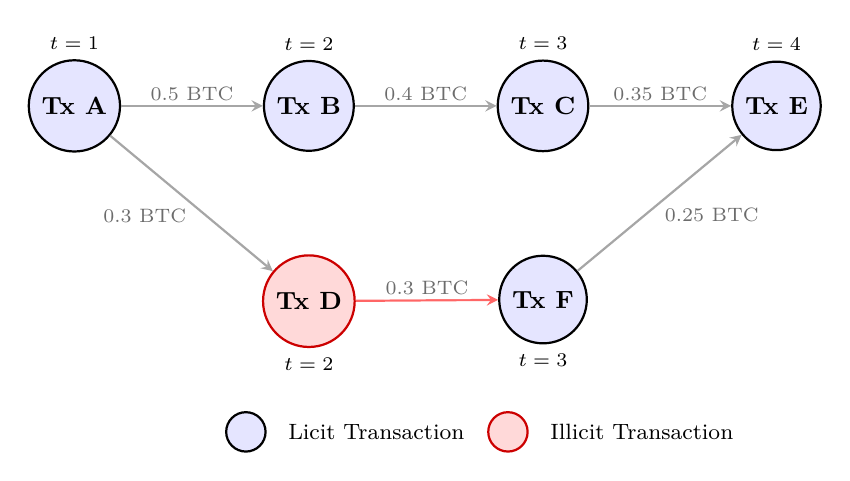
\begin{tikzpicture}[
    node distance=1.3cm and 1.8cm,
    txnode/.style={circle, draw=black, fill=blue!10, thick, minimum size=1.0cm, font=\small\bfseries},
    illicit/.style={circle, draw=red!80!black, fill=red!15, thick, minimum size=1.0cm, font=\small\bfseries},
    edge/.style={->, >=stealth, thick, draw=gray!70},
    illicitedge/.style={->, >=stealth, thick, draw=red!60},
    tlabel/.style={font=\scriptsize, text=gray!85!black, fill=white, inner sep=1.5pt, rounded corners=1pt},
]
% Nodes
\node[txnode, label=above:{\scriptsize $t=1$}] (A) {Tx A};
\node[txnode, right=of A, label=above:{\scriptsize $t=2$}] (B) {Tx B};
\node[txnode, right=of B, label=above:{\scriptsize $t=3$}] (C) {Tx C};
\node[illicit, below=of B, label=below:{\scriptsize $t=2$}] (D) {Tx D};
\node[txnode, right=of C, label=above:{\scriptsize $t=4$}] (E) {Tx E};
\node[txnode, below=of C, label=below:{\scriptsize $t=3$}] (F) {Tx F};

% Edges
\draw[edge] (A) -- (B) node[midway, above, tlabel] {0.5 BTC};
\draw[edge] (A) -- (D) node[midway, below left, tlabel] {0.3 BTC};
\draw[edge] (B) -- (C) node[midway, above, tlabel] {0.4 BTC};
\draw[illicitedge] (D) -- (F) node[midway, above, tlabel] {0.3 BTC};
\draw[edge] (C) -- (E) node[midway, above, tlabel] {0.35 BTC};
\draw[edge] (F) -- (E) node[midway, below right, tlabel] {0.25 BTC};

% Legend placed below the diagram
\node[txnode, minimum size=0.5cm, below=0.8cm of D, xshift=-0.8cm] (leg1) {};
\node[right=0.15cm of leg1, font=\footnotesize] {Licit Transaction};
\node[illicit, minimum size=0.5cm, right=2.8cm of leg1] (leg2) {};
\node[right=0.15cm of leg2, font=\footnotesize] {Illicit Transaction};
\end{tikzpicture}
\caption[Conceptual Bitcoin Transaction Network]{Conceptual illustration of a Bitcoin transaction network. Nodes represent transactions; directed edges represent UTXO fund flows with associated BTC amounts. Time step labels ($t$) indicate the temporal ordering. Red nodes represent illicit transactions identified through forensic analysis.}
\label{fig:bitcoin_concept}
\end{figure}

---

\section{Need Analysis}
\label{sec:intro_need}

\subsection{Limitations of Conventional AML Approaches}
\label{subsec:limitations}

Conventional approaches to Anti-Money Laundering in cryptocurrency networks suffer from several critical limitations that motivate the proposed research:

\begin{enumerate}
	\item \textbf{Static Graph Modelling:} Methods based on Graph Convolutional Networks (GCN)~\cite{kipf2017gcn}, Graph Attention Networks (GAT)~\cite{velivckovic2018gat}, and GraphSAGE~\cite{hamilton2017graphsage} treat the transaction graph as a fixed, time-invariant structure. This collapses the temporal dimension and destroys the sequential fund flow information that is central to detecting layering chains and other velocity-dependent laundering patterns.

	\item \textbf{Temporal Data Leakage:} When static GNNs are applied to temporal graphs using random train/test splits, the model aggregates feature information from future transactions to predict past ones. This introduces artificial performance inflation that does not generalise to real-time deployment, where only historical transaction data is available at inference time.

	\item \textbf{Fixed Temporal Encoding:} Some recent approaches introduce discrete temporal graph snapshots or fixed sinusoidal time encodings (inspired by NLP Transformers~\cite{vaswani2017attention}). Fixed-frequency sinusoids assume periodic, uniform temporal distributions, which do not reflect the non-stationary, bursty, power-law transaction patterns observed in cryptocurrency networks.

	\item \textbf{Binary Classification Only:} The overwhelming majority of AML GNN literature~\cite{weber2019anti, pareja2020evolvegcn} produces only a binary illicit/licit classification label. This is insufficient for regulatory compliance, which requires identification of the \textit{specific laundering typology} (circular transfer, layering, smurfing) and traceable evidence subgraphs for SAR filing.

	\item \textbf{Lack of Explainability:} Models that produce a scalar risk score without accompanying evidence are not actionable for compliance officers. Financial regulators increasingly require that AML alerts be accompanied by auditable, human-interpretable evidence trails~\cite{giese2022explainable}.

	\item \textbf{No Pattern-Level Investigation Evidence:} Existing methods do not isolate the specific transaction sub-network responsible for the alert, making it impossible to generate an investigation-ready SAR without manual forensic analysis.
\end{enumerate}

These gaps collectively define the research problem addressed in this dissertation.

\subsection{Importance of Anti-Money Laundering}
\label{subsec:importance_aml}

Anti-Money Laundering (AML) frameworks are foundational to the integrity of global financial systems. The Financial Action Task Force (FATF) reports that between 2\% and 5\% of global GDP—approximately \$800 billion to \$2 trillion—is laundered annually~\cite{fatf2022}. In the cryptocurrency domain, illicit transaction volume reached an all-time high of \$20.6 billion in 2022 and remained elevated at \$24.2 billion in 2023~\cite{chainalysis2023}, driven primarily by sanctions evasion, darknet market activity, and ransomware payments.

\subsection{Why Existing Tools Fall Short}
\label{subsec:shortcomings}

Current industry AML compliance relied heavily on:
\begin{enumerate}
    \item \textbf{Rule-Based Threshold Systems:} Systems triggering alerts when transaction values exceed arbitrary limits (e.g., \$10,000) are easily circumvented through \textit{smurfing}—splitting large sums into dozens of sub-threshold transactions across multiple wallets.
    \item \textbf{Tabular Machine Learning Models:} Classifiers (Random Forests, XGBoost) operating on isolated transaction attributes evaluate each transfer out of its topological context. They fail to identify laundering that is evident only when examining multi-hop chains or cycles.
    \item \textbf{Static Graph Neural Networks:} Graph Convolutional Networks (GCN) and Graph Attention Networks (GAT) capture topology but treat the entire transaction graph as an unweighted, static entity. They aggregate past and future edges interchangeably, causing catastrophic \textit{temporal leakage} in evaluation and failing to model the velocity and sequencing of fund transfers.
    \item \textbf{Opaque Binary Predictions:} High false-positive rates ($>90\%$ in standard compliance pipelines) overwhelm compliance analysts. Without interpretable, evidentiary subgraphs detailing \textit{which} multi-hop path constituted the suspicious typology, alerts cannot be effectively translated into actionable Suspicious Activity Reports (SARs).
\end{enumerate}

\subsection{Research Gap}
\label{subsec:research_gap}

Table~\ref{tab:research_gap} summarises the key research gaps identified from a systematic review of the literature.

\begin{table}[!htbp]
\centering
\caption[Research Gap Summary]{Summary of research gaps in existing AML and graph neural network literature.}
\label{tab:research_gap}
\small
\begin{tabularx}{\textwidth}{>{\hsize=0.85\hsize}L >{\hsize=0.95\hsize}L >{\hsize=1.1\hsize}L >{\hsize=1.1\hsize}L}
\toprule
\textbf{Approach} & \textbf{Representative Works} & \textbf{Contribution} & \textbf{Research Gap} \\
\midrule
Static GCN-based AML & Weber et al.~\cite{weber2019anti}; Pareja et al.~\cite{pareja2020evolvegcn} & Binary illicit classification on Elliptic dataset & Static graph; no temporal ordering; future data leakage \\
Graph Attention Networks & Veli\v{c}kovi\'{c} et al.~\cite{velivckovic2018gat}; Hu et al.~\cite{hu2020gat} & Attention-weighted neighbourhood aggregation & No temporal dimension; edge timestamps ignored \\
GraphSAGE & Hamilton et al.~\cite{hamilton2017graphsage} & Inductive neighbourhood sampling & No time encoding; treats graph as static \\
GNN-LSTM Hybrids & Pareja et al.~\cite{pareja2020evolvegcn}; Kim et al.~\cite{kim2022gnn} & Combines GNN spatial aggregation with LSTM temporal modelling & Temporal and spatial modules are decoupled; no continuous time encoding in attention \\
Dynamic/Temporal GNN & Xu et al.~\cite{xu2020tgat}; Rossi et al.~\cite{rossi2020tgn} & Continuous-time graph attention with temporal encoding & Fixed sinusoidal frequencies; not tuned to cryptocurrency transaction dynamics \\
Explainable AML & Giese et al.~\cite{giese2022explainable}; Lo et al.~\cite{lo2023gnn} & GNN explanations for financial fraud & Binary labels only; no pattern-level evidence extraction \\
Fixed-Frequency Temporal & Vaswani et al.~\cite{vaswani2017attention}; Xu et al.~\cite{xu2020tgat} & Sinusoidal position encoding for uniform sequences & Frequencies are geometrically fixed; cannot adapt to bursty cryptocurrency intervals \\
\midrule
\textbf{TemporalAML (Proposed)} & \textbf{This dissertation} & \textbf{Learnable Fourier encoding + multi-pattern TGAT + GNNExplainer} & \textbf{Addresses all above gaps} \\
\bottomrule
\end{tabularx}
\end{table}

---

\section{Problem Identification}
\label{sec:intro_problem}

\subsection{Problem Statement}
\label{subsec:problem_statement}

Existing Anti-Money Laundering methods for cryptocurrency transaction networks are constrained by static graph representations that discard temporal ordering, fixed-frequency time encodings that cannot adapt to bursty transaction dynamics, binary classification outputs that fail to identify specific laundering typologies, and the absence of per-alert explainable subgraph evidence. These limitations collectively prevent existing systems from satisfying the operational requirements of modern financial compliance.

\vspace{0.5em}
\noindent\textbf{Formal Problem Statement:} \\[0.5em]
\textit{Given a directed, weighted, temporal Bitcoin transaction graph $G = (V, E, \mathbf{X}, \mathbf{T})$, where $V$ is the set of transaction nodes, $E$ is the set of directed UTXO fund-flow edges, $\mathbf{X} \in \mathbb{R}^{|V| \times d}$ is the node feature matrix, and $\mathbf{T}$ is the set of chronologically ordered transaction timestamps: design a temporal graph attention model that (i) learns from continuous transaction time deltas through trainable Fourier frequency parameters embedded in the attention mechanism; (ii) simultaneously detects three distinct structural laundering typologies—Circular Transfers, Layering Chains, and Smurfing/Fan-Out behaviour—using shared temporal graph representations; and (iii) generates per-alert, per-pattern, time-ordered subgraph evidence sufficient for regulatory SAR investigation, without relying on future transaction data during inference.}

---

\section{Problem Formulation}
\label{sec:intro_formulation}

\subsection{Motivation}
\label{subsec:motivation}

The convergence of three trends motivates this research:

\begin{enumerate}
	\item \textbf{Scale of Cryptocurrency Laundering:} Global AML non-compliance fines exceeded \$10.4 billion in 2020 alone, while cryptocurrency-specific laundering is projected to grow with the increasing adoption of decentralised finance (DeFi) platforms~\cite{chainalysis2023}. Automated systems capable of operating at blockchain scale (millions of transactions) are essential.

	\item \textbf{Maturity of Temporal Graph Learning:} Recent advances in continuous-time graph neural networks (TGAT~\cite{xu2020tgat}, TGN~\cite{rossi2020tgn}) have demonstrated the feasibility of embedding temporal information directly into graph attention mechanisms. These methods, however, have not been applied to multi-pattern AML detection with explainability requirements.

	\item \textbf{Regulatory Demand for Explainable AML:} The Financial Action Task Force (FATF) and national regulators increasingly require that automated AML systems provide auditable, human-interpretable justification for alerts. Model explainability frameworks such as GNNExplainer~\cite{ying2019gnnexplainer} offer a principled mechanism for generating subgraph evidence that compliance officers can review and act upon.
\end{enumerate}

\subsection{Research Aim}
\label{subsec:aim}

\begin{quote}
\textit{To design, implement, and validate a Temporal Graph Attention Network with learnable Fourier time encoding for explainable multi-pattern Anti-Money Laundering detection in cryptocurrency transaction networks.}
\end{quote}

\subsection{Objectives}
\label{subsec:objectives}

The research is structured around four specific technical objectives:

\begin{enumerate}
	\item[\textbf{O1}] \textbf{Temporal Graph Construction:} Build a directed, weighted, temporal graph from the Elliptic Bitcoin Dataset, representing transaction entities as nodes and timestamped UTXO flows as directed edges, while preserving the 49 ordered time snapshots and enforcing strictly chronological, leakage-free data splitting.

	\item[\textbf{O2}] \textbf{Learnable Fourier Time Encoding:} Design and implement trainable Fourier frequency parameters ($\boldsymbol{\omega}$) and phase shifts ($\boldsymbol{\phi}$) inside the graph attention mechanism to allow the model to learn the characteristic temporal patterns of cryptocurrency laundering transactions through end-to-end gradient descent.

	\item[\textbf{O3}] \textbf{Unified Multi-Pattern Detection:} Develop pattern-specific detection mechanisms on shared temporal graph representations for three structural AML typologies: (a) Circular Transfers, (b) Layering Chains, and (c) Smurfing/Fan-Out behaviour, using a multi-task joint loss.

	\item[\textbf{O4}] \textbf{Per-Pattern Subgraph Explainability:} Integrate GNNExplainer to generate time-ordered, pattern-specific subgraph evidence for individual AML alerts, supporting regulatory SAR filing requirements.
\end{enumerate}

\noindent \textbf{Objective 5 (Future Work):} Comprehensive benchmarking against GCN, GraphSAGE, GNN-LSTM, and static GAT baselines with full F1, AUC-ROC, precision/recall, ablation, and temporal robustness evaluation is planned for Dissertation Phase~2.

\subsection{Scope of the Study}
\label{subsec:scope}

\textbf{Phase 1 Scope (this report):}
\begin{itemize}
	\item Complete design and implementation of the temporal graph construction pipeline (O1).
	\item Full implementation of the Learnable Fourier Time Encoding module and its integration into the TGAT attention mechanism (O2).
	\item Design and preliminary implementation of the shared-embedding multi-pattern TGAT with three classification heads (O3).
	\item Design and implementation of the GNNExplainer-based per-pattern subgraph explanation pipeline (O4).
	\item Dataset: Elliptic Bitcoin Dataset (203,769 nodes, 234,355 edges, 49 time steps, 166 raw features).
\end{itemize}

\textbf{Deferred to Phase 2:}
\begin{itemize}
	\item Full model training to convergence with hyperparameter tuning.
	\item Systematic benchmarking against baseline models (GCN, GraphSAGE, GNN-LSTM, static GAT).
	\item Comprehensive evaluation: F1-score, AUC-ROC, precision, recall, AUPRC.
	\item Ablation study isolating the contribution of each module.
	\item Temporal robustness and cross-time-step generalisation evaluation.
	\item Explainability quality evaluation (fidelity, sparsity, SAR generation quality).
\end{itemize}

\subsection{Expected Contributions}
\label{subsec:contributions}

The expected contributions of this dissertation are:
\begin{enumerate}
	\item \textbf{A novel Learnable Fourier Time Encoding module} that adapts sinusoidal frequency parameters through gradient descent to capture the non-stationary, bursty temporal dynamics of cryptocurrency transactions—distinguishing it from fixed-frequency encodings used in prior temporal GNN work.
	\item \textbf{A unified multi-task TGAT architecture} that simultaneously detects three structural money laundering patterns (Circular Transfers, Layering Chains, Smurfing) from a shared 128-dimensional latent node representation, avoiding the computational cost and information isolation of training three separate models.
	\item \textbf{A per-pattern, time-ordered, GNNExplainer-based evidence subgraph pipeline} that generates investigation-ready transaction chains for each detected laundering alert, directly addressing the explainability gap in existing cryptocurrency AML systems.
	\item \textbf{A strictly leakage-free temporal data pipeline} with chronological graph splitting, causal temporal neighbourhood sampling, and training-only feature normalisation, establishing a principled evaluation protocol for temporal AML research.
\end{enumerate}

\chapter{LITERATURE SURVEY AND OBJECTIVES}
\label{ChapterLiteratureSurvey}

\section{Critical Review of Literature}
\label{sec:critical_review}

A systematic review of the literature reveals a clear trajectory from rule-based AML heuristics to static graph neural networks and, more recently, towards temporal and explainable graph learning. This section critically examines the major methodological streams relevant to this dissertation.

\subsection{Anti-Money Laundering using Graph Convolutional Networks}

Weber et al.~\cite{weber2019anti} introduced the application of GCNs to the Elliptic Bitcoin Dataset, demonstrating that graph-based methods significantly outperform traditional tabular classifiers (Random Forest, Logistic Regression) on the binary illicit/licit classification task. Their seminal work established the Elliptic dataset as the standard benchmark for cryptocurrency AML research and reported F1-scores of approximately 0.70 for the illicit class. However, their approach treats the graph as a single static snapshot, making it vulnerable to temporal data leakage and unable to exploit the sequential nature of fund flows.

Subsequent work~\cite{pareja2020evolvegcn} proposed EvolveGCN, which evolves GCN weights over time using a Gated Recurrent Unit (GRU), enabling the model to adapt its parameters across discrete graph snapshots. While EvolveGCN represents a meaningful step toward temporal modelling, it still operates on \textit{discrete} graph snapshots rather than continuous transaction timestamps, losing sub-interval temporal velocity information that is critical for detecting rapid layering chains.

\subsection{Graph Attention Networks}

The Graph Attention Network (GAT) architecture~\cite{velivckovic2018gat} introduced learnable attention coefficients into the neighbourhood aggregation process, allowing nodes to assign differentiated importance to their neighbours. Unlike GCNs, which use fixed symmetric normalisation, GAT adaptively weights neighbourhood features, making it theoretically better suited to heterogeneous financial transaction graphs where not all neighbours are equally informative. However, standard GAT does not incorporate edge timestamps, treating all neighbours as equally contemporaneous regardless of their temporal distance from the target node.

Hu et al.~\cite{hu2020gat} applied attention-based GNNs to fraud detection in financial networks, demonstrating that attention mechanisms can isolate structurally suspicious nodes. Their work, however, focuses on static social/financial graphs without temporal components.

\subsection{GraphSAGE and Inductive Learning}

Hamilton et al.~\cite{hamilton2017graphsage} proposed GraphSAGE (SAmple and agGrEgate), an inductive graph learning framework that samples a fixed-size neighbourhood for each node and applies learnable aggregator functions. GraphSAGE's inductive capability—allowing inference on unseen nodes without retraining—is important for real-time AML systems where new transactions continuously enter the graph. Weber et al.~\cite{weber2019anti} included GraphSAGE as a baseline on the Elliptic dataset. GraphSAGE achieves competitive performance but, like GCN and GAT, ignores edge timestamps.

\subsection{Temporal Graph Networks}

Rossi et al.~\cite{rossi2020tgn} proposed the Temporal Graph Network (TGN) framework, which maintains a dynamic memory state for each node updated by observed interactions over continuous time. TGN represents the state of the art in general temporal graph learning and enables the model to recall long-term historical interaction patterns. However, TGN's memory module introduces substantial computational overhead and requires additional memory storage per node, which scales poorly to graphs with hundreds of thousands of transaction nodes.

\subsection{Temporal Graph Attention Networks (TGAT)}

Xu et al.~\cite{xu2020tgat} proposed TGAT, which integrates continuous-time temporal encoding into a self-attention mechanism inspired by the Transformer architecture~\cite{vaswani2017attention}. TGAT uses fixed harmonic sinusoidal functions to project time differences $\Delta t$ into a vector space, which is then concatenated with node features before attention computation. TGAT has demonstrated strong performance on social interaction and bipartite graphs. The critical limitation, however, is that TGAT's sinusoidal frequencies are \textit{geometrically fixed} (following the standard Transformer formula $\omega_i = 10000^{-2i/d}$), which is calibrated for natural language token sequences—not for the non-stationary, power-law distributed transaction intervals of cryptocurrency networks.

\subsection{GNN-LSTM Hybrid Approaches}

Several works have combined GNN spatial aggregation with LSTM temporal modelling. Kim et al.~\cite{kim2022gnn} applied a GNN-LSTM hybrid to anti-money laundering on synthetic transaction graphs, demonstrating that hybrid architectures capture both structural and sequential patterns. The fundamental limitation is architectural coupling: the GNN processes structure and the LSTM processes sequences as separate modules, meaning that temporal information does not directly influence the neighbourhood attention weighting. In contrast, TemporalAML embeds temporal information \textit{directly into the attention coefficient} $\alpha_{ij}$, allowing temporal distance to modulate how much structural information is propagated from each neighbour.

\subsection{Wavelet and Frequency-Based Temporal Graph Approaches}

Some recent works have explored spectral and frequency-based approaches to temporal graph modelling. Bochner's Theorem~\cite{bochner1933monotone} provides a theoretical foundation: any continuous, shift-invariant kernel can be represented as the Fourier transform of a positive measure. This justifies the use of sinusoidal basis functions for temporal encoding. The key insight of TemporalAML's O2 is to make the Fourier frequencies \textit{learnable} via gradient descent rather than fixing them geometrically, allowing the model to discover the transaction-specific frequency components most relevant to laundering detection.

\subsection{Explainable GNN Approaches for AML}

Ying et al.~\cite{ying2019gnnexplainer} introduced GNNExplainer, a model-agnostic method that learns a soft edge mask $M \in [0,1]^{|E_s|}$ by maximising the mutual information between the prediction of the full graph and a compact subgraph. GNNExplainer identifies the minimal transaction sub-network most responsible for a classification decision, directly supporting the generation of investigation-ready evidence.

Giese et al.~\cite{giese2022explainable} applied explainability frameworks to financial fraud detection, demonstrating that node and edge importance scores can meaningfully identify suspicious transaction chains. Lo et al.~\cite{lo2023gnn} extended GNN explainability to cryptocurrency fraud detection, but their work focuses on binary labels without pattern-specific evidence extraction. TemporalAML addresses this by linking explainability to specific typology heads (Circular, Layering, Smurfing), producing \textit{per-pattern} evidence subgraphs rather than generic node importances.

---

\section{Literature Collection and Segregation}
\label{sec:lit_collection}

Table~\ref{tab:lit_review} presents a structured synthesis of the key works surveyed, classifying them by methodology, dataset, contribution, and identified research gap.

\begingroup
\setlength{\tabcolsep}{3pt}
\footnotesize
\renewcommand{\arraystretch}{1.2}
\begin{longtable}{@{} c p{2.7cm} p{1.7cm} c p{1.3cm} p{1.5cm} p{2.1cm} p{2.1cm} @{}}
\caption[Literature Review Table]{Structured literature review of methods relevant to AML and temporal graph learning.}
\label{tab:lit_review}\\
\toprule
\textbf{\#} & \textbf{Paper Title} & \textbf{Authors} & \textbf{Yr} & \textbf{Dataset} & \textbf{Method} & \textbf{Key Contribution} & \textbf{Limitation / Gap} \\
\midrule
\endfirsthead

\toprule
\textbf{\#} & \textbf{Paper Title} & \textbf{Authors} & \textbf{Yr} & \textbf{Dataset} & \textbf{Method} & \textbf{Key Contribution} & \textbf{Limitation / Gap} \\
\midrule
\endhead

\bottomrule
\endfoot

\bottomrule
\endlastfoot

1 & Anti-Money Laundering in Bitcoin: Experimenting with GNNs & Weber et al. & 2019 & Elliptic Bitcoin & GCN, LogReg, RF & First GNN baseline on Elliptic; binary classification & Static graph; future data leakage; binary only \\
\addlinespace
2 & EvolveGCN: Evolving GCN for Dynamic Graphs & Pareja et al. & 2020 & Elliptic, Reddit & GRU-evolved GCN weights & Temporal GCN evolving parameters over snapshots & Discrete snapshots; no continuous time encoding \\
\addlinespace
3 & Graph Attention Networks & Veli\v{c}kovi\'{c} et al. & 2018 & Cora, Citeseer & Multi-head attention GAT & Learnable attention over neighbours & No temporal awareness; static edges \\
\addlinespace
4 & Inductive Representation Learning on Large Graphs & Hamilton et al. & 2017 & Reddit, PPI & GraphSAGE aggregation & Inductive node classification & No time encoding; static graph assumption \\
\addlinespace
5 & Inductive Representation for Temporal Graphs (TGAT) & Xu et al. & 2020 & Wikipedia, Reddit & Fixed sinusoidal Fourier + self-attention & Continuous-time temporal graph attention & Fixed frequencies; not tuned to financial data \\
\addlinespace
6 & Temporal Graph Networks & Rossi et al. & 2020 & Wikipedia, Twitter & Memory + message passing & Dynamic node state with temporal memory & High memory overhead; complex training \\
\addlinespace
7 & GNNExplainer & Ying et al. & 2019 & BA-Shapes, Mutagenicity & Mutual info edge mask optimisation & Model-agnostic subgraph explainability & No per-pattern; no temporal subgraph ordering \\
\addlinespace
8 & Explainable AI for Financial Fraud & Giese et al. & 2022 & Synthetic financial & XAI + GNN & Compliance-oriented fraud explanations & Binary labels; no crypto-specific typologies \\
\addlinespace
9 & GNN for AML in Cryptocurrency & Lo et al. & 2023 & Ethereum & Graph classification + SHAP & Cryptocurrency fraud GNN with attribution & No pattern-level evidence; no temporal encoding \\
\addlinespace
10 & GNN-LSTM for AML & Kim et al. & 2022 & Synthetic AML & GCN + LSTM & Hybrid spatial-temporal architecture & Decoupled time and structure; no attention-time fusion \\
\addlinespace
11 & Attention is All You Need & Vaswani et al. & 2017 & WMT EN-DE & Transformer self-attention & Fixed sinusoidal positional encoding & Non-learnable frequencies; NLP-specific design \\
\addlinespace
12 & Benchmarking GNNs & Dwivedi et al. & 2020 & Multiple benchmarks & GCN, GAT, GIN & Comprehensive GNN performance analysis & Financial and temporal graphs not included \\
\addlinespace
13 & Elliptic Dataset & Elliptic / MIT-IBM & 2019 & Elliptic Bitcoin & Dataset paper & 203,769-node labelled Bitcoin graph (49 time steps) & No temporal model proposed; binary only \\
\addlinespace
14 & Semi-Supervised Classification with GCN & Kipf \& Welling & 2017 & Cora, Citeseer & Spectral GCN & Foundational GCN for node classification & No temporal dimension; transductive only \\
\addlinespace
15 & Graph Neural Networks for AML & Johannessen et al. & 2023 & Banking data & GNN + rules & GNN applied to banking transaction AML & Not cryptocurrency-specific; no explainability \\
\end{longtable}
\endgroup

---

\section{Summary of Literature}
\label{sec:lit_summary}

The reviewed literature reveals a clear progression: early works established GNNs as effective tools for cryptocurrency AML (Weber et al.~\cite{weber2019anti}), but these approaches treat the transaction graph as a static structure. Subsequent works introduced temporal modelling through discrete graph snapshots (EvolveGCN~\cite{pareja2020evolvegcn}) and continuous-time attention (TGAT~\cite{xu2020tgat}, TGN~\cite{rossi2020tgn}), but none have applied learnable frequency-based temporal encoding to the specific domain of cryptocurrency AML. The explainability stream (GNNExplainer~\cite{ying2019gnnexplainer}, Giese et al.~\cite{giese2022explainable}) has demonstrated the feasibility of subgraph evidence extraction but has not been applied to pattern-specific, time-ordered AML evidence generation.

No existing work simultaneously addresses: (i) continuous learnable temporal encoding within graph attention, (ii) multi-pattern laundering typology detection, and (iii) per-pattern GNNExplainer evidence subgraph generation. TemporalAML is designed to fill this gap.

---

\section{Identification of Gaps}
\label{sec:gaps}

Based on the literature review, the following specific research gaps are identified:

\begin{enumerate}
	\item \textbf{Static graph representations:} GCN, GAT, and GraphSAGE-based AML models discard temporal ordering, leading to data leakage and inability to detect velocity-dependent laundering patterns.
	\item \textbf{Fixed temporal encoding:} TGAT uses geometrically fixed sinusoidal frequencies that are not tuned to cryptocurrency transaction intervals; EvolveGCN uses discrete snapshots that lose sub-interval temporal information.
	\item \textbf{Binary-only classification:} No existing cryptocurrency AML GNN simultaneously identifies multiple structural laundering typologies from shared graph representations.
	\item \textbf{Absence of per-pattern explainability:} No prior work generates time-ordered, per-pattern subgraph evidence specifically for cryptocurrency laundering alerts.
	\item \textbf{Temporal data leakage in evaluation protocols:} Many existing studies use random train/test splits on temporal graphs, inflating reported performance metrics.
\end{enumerate}

---

\section{Need for Research}
\label{sec:need_for_research}

The identified gaps collectively motivate the need for a new framework that: (i) respects the continuous temporal structure of cryptocurrency transaction graphs; (ii) learns the characteristic time-frequency components of laundering behaviour in a data-driven manner; (iii) detects multiple structural laundering patterns simultaneously; and (iv) provides investigation-ready explainability for regulatory compliance. TemporalAML is designed to address each of these needs within a unified end-to-end framework.

---

\section{Problem Statement}
\label{sec:lit_problem_statement}

Existing anti-money laundering systems for cryptocurrency transaction networks cannot simultaneously detect multiple structural laundering typologies—Circular Transfers, Layering Chains, and Smurfing/Fan-Out behaviour—from continuous temporal graph representations, nor generate per-pattern, time-ordered, explainable subgraph evidence required for regulatory SAR filing, without introducing temporal data leakage. This research proposes TemporalAML, a Temporal Graph Attention Network with learnable Fourier time encoding, to address these limitations.

---

\section{Objectives}
\label{sec:lit_objectives}

\begin{enumerate}
	\item[\textbf{O1}] Construct a directed, weighted, temporal graph $G = (V, E, \mathbf{X}, \mathbf{T})$ from the Elliptic Bitcoin Dataset with 203,769 transaction nodes, 234,355 directed edges, 172 features per node (including six engineered topological attributes), and 49 ordered time snapshots, with a strictly chronological leakage-free data split.
	
	\item[\textbf{O2}] Design and implement a Learnable Fourier Time Encoding module with trainable frequency parameters $\boldsymbol{\omega} \in \mathbb{R}^{d/2}$ and phase shifts $\boldsymbol{\phi} \in \mathbb{R}^{d/2}$ integrated into the temporal graph attention mechanism, enabling end-to-end gradient-driven adaptation to cryptocurrency transaction velocity patterns.
	
	\item[\textbf{O3}] Develop a two-layer Temporal Graph Attention Network (TGAT) with a shared 128-dimensional latent representation backbone and three parallel pattern-specific classification heads for Circular Transfer, Layering Chain, and Smurfing detection, trained via a joint class-weighted multi-task binary cross-entropy loss.
	
	\item[\textbf{O4}] Integrate GNNExplainer to optimise per-alert edge masks $M \in [0,1]^{|E_s|}$ by maximising mutual information, generating minimal time-ordered pattern-specific subgraph evidence for regulatory SAR filing.
\end{enumerate}

\noindent \textit{Note: Objective 5 — Comprehensive benchmarking and validation against GCN, GraphSAGE, GNN-LSTM, and static GAT baselines — is planned for Dissertation Phase 2.}

---

\section{Limitations of the Study}
\label{sec:limitations}

As an academic research project conducted in Dissertation Phase~1, the following limitations apply:

\begin{enumerate}
	\item \textbf{Dataset scope:} This research uses only the Elliptic Bitcoin Dataset. Generalisation to other cryptocurrencies (Ethereum, Monero) or other financial graph datasets is not evaluated in Phase~1.

	\item \textbf{Transaction-level representation:} The Elliptic dataset represents transactions as nodes, not wallet addresses. As a result, Circular Transfers — which at the wallet-graph level correspond to fund cycles — cannot form closed cycles at the Bitcoin transaction-level graph, which is a strict Directed Acyclic Graph (DAG). This is a domain constraint of the dataset rather than a limitation of the method, and is documented explicitly in the methodology.

	\item \textbf{Unsupervised pattern label mining:} Ground-truth labels for Layering and Smurfing patterns are derived through graph-theoretic mining (BFS and degree thresholding) applied to the illicit node subgraph, rather than from forensic investigator annotations. This introduces label noise that may affect pattern detection precision.

	\item \textbf{Benchmarking deferred:} Systematic comparison against GCN, GraphSAGE, GNN-LSTM, and other baselines, along with F1, AUC-ROC, ablation, and temporal robustness evaluation, is planned for Phase~2.

	\item \textbf{Explainability evaluation deferred:} Qualitative and quantitative evaluation of GNNExplainer output quality (fidelity, sparsity, SAR usability) is deferred to Phase~2.
\end{enumerate}

\chapter{PROPOSED METHODOLOGY}
\label{ChapterResearchMethodology}

This chapter presents the complete technical methodology of TemporalAML, covering the dataset, preprocessing pipeline, temporal graph construction, learnable Fourier time encoding, Temporal Graph Attention Network architecture, multi-pattern AML detection heads, and per-pattern subgraph explainability. The chapter is structured to follow the four research objectives.

---

\section{Problem Formulation}
\label{sec:meth_problem}

Let $G = (V, E, \mathbf{X}, \mathbf{T})$ denote the directed, weighted, temporal transaction graph, where:
\begin{itemize}
	\item $V = \{v_1, v_2, \ldots, v_N\}$ is the set of $N = 203{,}769$ transaction nodes.
	\item $E \subseteq V \times V$ is the set of $|E| = 234{,}355$ directed edges, where $(v_i, v_j) \in E$ indicates that transaction $v_i$ transferred funds to transaction $v_j$.
	\item $\mathbf{X} \in \mathbb{R}^{N \times d}$ is the node feature matrix, where $d = 172$ (166 raw features + 6 engineered features).
	\item $\mathbf{T} = \{t_{v_1}, t_{v_2}, \ldots, t_{v_N}\}$ is the set of integer time step labels $t \in [1, 49]$ assigned to each transaction node based on its blockchain confirmation snapshot.
\end{itemize}

\noindent The research objective is to learn a function:
\begin{equation}
f: G \rightarrow \left\{ \hat{y}^{\text{circ}}_v, \; \hat{y}^{\text{lay}}_v, \; \hat{y}^{\text{smurf}}_v \right\}_{v \in V}
\end{equation}
where $\hat{y}^{\text{circ}}_v, \hat{y}^{\text{lay}}_v, \hat{y}^{\text{smurf}}_v \in [0, 1]$ are the predicted probabilities that node $v$ is involved in a Circular Transfer, Layering Chain, or Smurfing pattern respectively, such that: (i) $f$ does not use future transaction information during inference; (ii) time differences $\Delta t = t_i - t_j$ are embedded via learnable Fourier parameters rather than fixed encodings; and (iii) for each alert, an explainability module identifies the minimal causal subgraph $G_s \subseteq G$ most responsible for the prediction.

---

\section{Proposed Research Framework}
\label{sec:meth_framework}

\subsection{Overall System Architecture}

Figure~\ref{fig:system_arch} illustrates the six-block modular system architecture of TemporalAML.

\begin{figure}[!htbp]
\centering
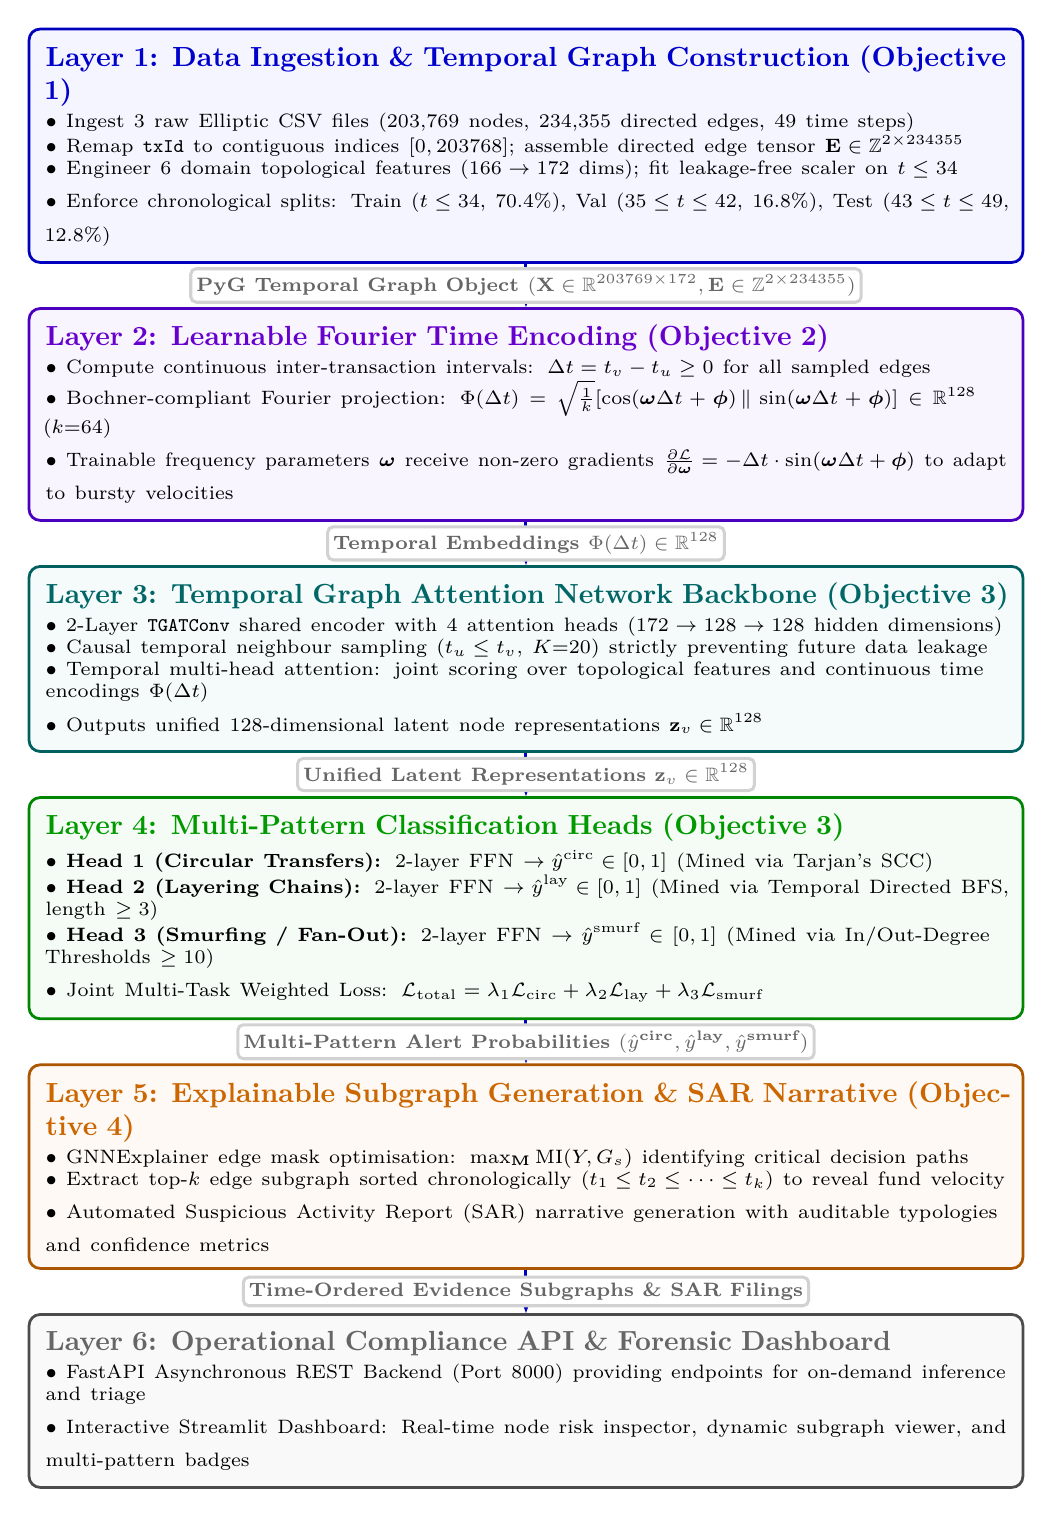
\begin{tikzpicture}[
    layer/.style={
        rectangle,
        draw=#1!75!black,
        fill=#1!4,
        line width=1.0pt,
        rounded corners=4pt,
        text width=12.2cm,
        inner sep=6pt,
        align=left
    },
    flowarrow/.style={
        ->,
        >={Stealth[length=2.5mm,width=1.8mm]},
        line width=1.1pt,
        draw=blue!75!black
    },
    flowtag/.style={
        fill=white,
        draw=gray!35,
        rounded corners=2pt,
        font=\scriptsize\bfseries,
        text=gray!80!black,
        inner sep=2pt
    }
]

% Layer 1
\node[layer=blue] (L1) at (0, 0) {
    \textcolor{blue!80!black}{\textbf{Layer 1: Data Ingestion \& Temporal Graph Construction (Objective 1)}}\\[2pt]
    \scriptsize $\bullet$ Ingest 3 raw Elliptic CSV files (203,769 nodes, 234,355 directed edges, 49 time steps)\\
    $\bullet$ Remap \texttt{txId} to contiguous indices $[0, 203768]$; assemble directed edge tensor $\mathbf{E} \in \mathbb{Z}^{2 \times 234355}$\\
    $\bullet$ Engineer 6 domain topological features ($166 \to 172$ dims); fit leakage-free scaler on $t \leq 34$\\
    $\bullet$ Enforce chronological splits: Train ($t \leq 34$, 70.4\%), Val ($35 \leq t \leq 42$, 16.8\%), Test ($43 \leq t \leq 49$, 12.8\%)
};

% Layer 2
\node[layer=blue!60!magenta, below=0.55cm of L1] (L2) {
    \textcolor{blue!50!magenta!80!black}{\textbf{Layer 2: Learnable Fourier Time Encoding (Objective 2)}}\\[2pt]
    \scriptsize $\bullet$ Compute continuous inter-transaction intervals: $\Delta t = t_v - t_u \geq 0$ for all sampled edges\\
    $\bullet$ Bochner-compliant Fourier projection: $\Phi(\Delta t) = \sqrt{\frac{1}{k}} [\cos(\boldsymbol{\omega}\Delta t + \boldsymbol{\phi}) \,\|\, \sin(\boldsymbol{\omega}\Delta t + \boldsymbol{\phi})] \in \mathbb{R}^{128}$ ($k{=}64$)\\
    $\bullet$ Trainable frequency parameters $\boldsymbol{\omega}$ receive non-zero gradients $\frac{\partial \mathcal{L}}{\partial \boldsymbol{\omega}} = -\Delta t \cdot \sin(\boldsymbol{\omega}\Delta t + \boldsymbol{\phi})$ to adapt to bursty velocities
};

% Layer 3
\node[layer=teal, below=0.55cm of L2] (L3) {
    \textcolor{teal!80!black}{\textbf{Layer 3: Temporal Graph Attention Network Backbone (Objective 3)}}\\[2pt]
    \scriptsize $\bullet$ 2-Layer \texttt{TGATConv} shared encoder with 4 attention heads ($172 \to 128 \to 128$ hidden dimensions)\\
    $\bullet$ Causal temporal neighbour sampling ($t_u \leq t_v$, $K{=}20$) strictly preventing future data leakage\\
    $\bullet$ Temporal multi-head attention: joint scoring over topological features and continuous time encodings $\Phi(\Delta t)$\\
    $\bullet$ Outputs unified 128-dimensional latent node representations $\mathbf{z}_v \in \mathbb{R}^{128}$
};

% Layer 4
\node[layer=green!70!black, below=0.55cm of L3] (L4) {
    \textcolor{green!60!black}{\textbf{Layer 4: Multi-Pattern Classification Heads (Objective 3)}}\\[2pt]
    \scriptsize $\bullet$ \textbf{Head 1 (Circular Transfers):} 2-layer FFN $\to \hat{y}^{\text{circ}} \in [0, 1]$ (Mined via Tarjan's SCC)\\
    $\bullet$ \textbf{Head 2 (Layering Chains):} 2-layer FFN $\to \hat{y}^{\text{lay}} \in [0, 1]$ (Mined via Temporal Directed BFS, length $\geq 3$)\\
    $\bullet$ \textbf{Head 3 (Smurfing / Fan-Out):} 2-layer FFN $\to \hat{y}^{\text{smurf}} \in [0, 1]$ (Mined via In/Out-Degree Thresholds $\geq 10$)\\
    $\bullet$ Joint Multi-Task Weighted Loss: $\mathcal{L}_{\text{total}} = \lambda_1 \mathcal{L}_{\text{circ}} + \lambda_2 \mathcal{L}_{\text{lay}} + \lambda_3 \mathcal{L}_{\text{smurf}}$
};

% Layer 5
\node[layer=orange!90!black, below=0.55cm of L4] (L5) {
    \textcolor{orange!80!black}{\textbf{Layer 5: Explainable Subgraph Generation \& SAR Narrative (Objective 4)}}\\[2pt]
    \scriptsize $\bullet$ GNNExplainer edge mask optimisation: $\max_{\mathbf{M}} \text{MI}(Y, G_s)$ identifying critical decision paths\\
    $\bullet$ Extract top-$k$ edge subgraph sorted chronologically ($t_1 \leq t_2 \leq \dots \leq t_k$) to reveal fund velocity\\
    $\bullet$ Automated Suspicious Activity Report (SAR) narrative generation with auditable typologies and confidence metrics
};

% Layer 6
\node[layer=gray!80!black, below=0.55cm of L5] (L6) {
    \textcolor{gray!80!black}{\textbf{Layer 6: Operational Compliance API \& Forensic Dashboard}}\\[2pt]
    \scriptsize $\bullet$ FastAPI Asynchronous REST Backend (Port 8000) providing endpoints for on-demand inference and triage\\
    $\bullet$ Interactive Streamlit Dashboard: Real-time node risk inspector, dynamic subgraph viewer, and multi-pattern badges
};

% Flow Arrows with Tags
\draw[flowarrow] (L1) -- node[flowtag] {PyG Temporal Graph Object $(\mathbf{X} \in \mathbb{R}^{203769 \times 172}, \mathbf{E} \in \mathbb{Z}^{2 \times 234355})$} (L2);
\draw[flowarrow] (L2) -- node[flowtag] {Temporal Embeddings $\Phi(\Delta t) \in \mathbb{R}^{128}$} (L3);
\draw[flowarrow] (L3) -- node[flowtag] {Unified Latent Representations $\mathbf{z}_v \in \mathbb{R}^{128}$} (L4);
\draw[flowarrow] (L4) -- node[flowtag] {Multi-Pattern Alert Probabilities $(\hat{y}^{\text{circ}}, \hat{y}^{\text{lay}}, \hat{y}^{\text{smurf}})$} (L5);
\draw[flowarrow] (L5) -- node[flowtag] {Time-Ordered Evidence Subgraphs \& SAR Filings} (L6);

\end{tikzpicture}
\caption[TemporalAML System Architecture]{Six-layer modular system architecture of TemporalAML. The end-to-end framework processes raw transaction data through temporal graph construction (O1), learnable Fourier time encoding (O2), a shared TGAT attention backbone (O3), multi-pattern classification heads (O3), and GNNExplainer evidence extraction (O4) to the interactive compliance dashboard. Rendered with clean academic styling on a white background.}
\label{fig:system_arch}
\end{figure}

---

\section{Data Collection and Preprocessing}
\label{sec:meth_data}

\subsection{Dataset Selection: The Elliptic Bitcoin Dataset}
\label{subsec:dataset_selection}

The \textbf{Elliptic Bitcoin Dataset}~\cite{elliptic2019} is the primary dataset used in this research. It is the only publicly available, large-scale, real-world, ground-truth-labelled Bitcoin transaction graph dataset, jointly published by Elliptic (a blockchain analytics firm) and the MIT--IBM Watson AI Lab. Table~\ref{tab:dataset_stats} provides the key dataset statistics.

\begin{table}[!htbp]
\centering
\caption[Elliptic Dataset Statistics]{Key statistics of the Elliptic Bitcoin Dataset.}
\label{tab:dataset_stats}
\begin{tabular}{lr}
\toprule
\textbf{Property} & \textbf{Value} \\
\midrule
Total Transaction Nodes ($|V|$) & 203,769 \\
Total Directed Edges ($|E|$) & 234,355 \\
Features per Transaction Node & 166 (raw) + 6 (engineered) = \textbf{172} \\
Temporal Snapshots (Time Steps) & 49 \\
Approximate Duration & 2 years of Bitcoin on-chain activity \\
Approx. Interval per Time Step & 2 weeks \\
\midrule
Labelled Nodes (Total) & 46,564 \\
Illicit Nodes & 4,545 (\textbf{2.2\%} of 203,769) \\
Licit Nodes & 42,019 (\textbf{20.6\%} of 203,769) \\
Unknown (Unlabelled) Nodes & 157,205 (\textbf{77.2\%} of 203,769) \\
\bottomrule
\end{tabular}
\end{table}

\vspace{0.5em}
\noindent \textbf{Relevance to AML:} The dataset contains Bitcoin transactions tagged by forensic investigators as associated with known illicit entities (darknet markets, ransomware operators, fraudulent exchanges). The temporal ordering of 49 time steps faithfully reflects the chronological evolution of on-chain activity, making it ideal for evaluating temporally-aware AML methods.

\subsection{Dataset Files}
\label{subsec:dataset_files}

Table~\ref{tab:dataset_files} describes the three CSV files constituting the Elliptic dataset.

\begin{table}[!htbp]
\centering
\caption[Elliptic Dataset File Descriptions]{Description of the three CSV files in the Elliptic Bitcoin Dataset.}
\label{tab:dataset_files}
\begin{tabularx}{\textwidth}{l c L}
\toprule
\textbf{File} & \textbf{Shape} & \textbf{Description} \\
\midrule
\texttt{elliptic\_txs\_features.csv} & 203,769 $\times$ 167 & Transaction node features. Column 0: Transaction ID (\texttt{txId}); Column 1: Time step $t \in [1, 49]$; Columns 2--95: 94 local features; Columns 96--167: 72 neighbourhood aggregation features. \\
\addlinespace
\texttt{elliptic\_txs\_edgelist.csv} & 234,355 $\times$ 2 & Directed fund-flow edges. Each row: (\texttt{txId1}, \texttt{txId2}) indicating that transaction \texttt{txId1} sent funds to transaction \texttt{txId2}. \\
\addlinespace
\texttt{elliptic\_txs\_classes.csv} & 203,769 $\times$ 2 & Ground-truth labels. Values: \texttt{1} (Illicit), \texttt{2} (Licit), \texttt{unknown}. \\
\bottomrule
\end{tabularx}
\end{table}

\subsection{Feature Structure}
\label{subsec:feature_structure}

Table~\ref{tab:feature_categories} describes the three categories of node features.

\begin{table}[!htbp]
\centering
\caption[Feature Category Breakdown]{Feature categories for each transaction node in the Elliptic dataset.}
\label{tab:feature_categories}
\begin{tabularx}{\textwidth}{l c L}
\toprule
\textbf{Feature Category} & \textbf{Dims} & \textbf{Description and Key Attributes} \\
\midrule
\textbf{Local Features} & 94 & Transaction-level attributes: fee (satoshis), total input/output BTC volume, input/output counts, byte size, time step $t$, mean input/output values, standard deviation of amounts. \\
\addlinespace
\textbf{Neighbourhood Features} & 72 & 1-hop aggregated statistics (mean, standard deviation, minimum, maximum) of local features over neighbouring transactions, capturing local graph context. \\
\addlinespace
\textbf{Engineered Topological} & 6 & Domain-specific features added in O1: out-degree, in-degree, fan-out ratio, fan-in ratio, temporal recency ($t/49$), mean neighbour time delta. \\
\midrule
\textbf{Total Feature Vector} & \textbf{172} & Concatenated feature vector per transaction node. \\
\bottomrule
\end{tabularx}
\end{table}

\subsection{Label Distribution}
\label{subsec:labels}

Table~\ref{tab:label_dist} summarises the class distribution. The severe class imbalance (2.2\% illicit) requires special handling through class-weighted loss functions.

\begin{table}[!htbp]
\centering
\caption[Label Distribution in Elliptic Dataset]{Class distribution in the Elliptic Bitcoin Dataset.}
\label{tab:label_dist}
\begin{tabularx}{\textwidth}{l r r L}
\toprule
\textbf{Class Label} & \textbf{Node Count} & \textbf{Percentage} & \textbf{Description} \\
\midrule
Illicit (Class 1) & 4,545 & 2.2\% & Transactions linked by forensic investigators to criminal entities (ransomware, darknet, fraud). \\
Licit (Class 2) & 42,019 & 20.6\% & Transactions from regulated entities (exchanges, miners, merchants). \\
Unknown & 157,205 & 77.2\% & Unlabelled transactions preserved in the graph to maintain full topological message-passing connectivity. \\
\midrule
\textbf{Total} & \textbf{203,769} & \textbf{100.0\%} & All transactions across 49 chronological time steps. \\
\bottomrule
\end{tabularx}
\end{table}

\subsection{Temporal Structure and Chronological Splits}
\label{subsec:temporal_structure}

Table~\ref{tab:temporal_splits} describes the 49-step temporal structure and the leakage-free chronological data split.

\begin{table}[!htbp]
\centering
\caption[Temporal Structure and Data Splits]{Temporal structure of the Elliptic dataset and the chronological data split protocol.}
\label{tab:temporal_splits}
\begin{tabular}{l l r r}
\toprule
\textbf{Split} & \textbf{Time Steps} & \textbf{Approx. Nodes} & \textbf{Percentage} \\
\midrule
Training & $t \in [1, 34]$ & 143,551 & 70.4\% \\
Validation & $t \in [35, 42]$ & 34,144 & 16.8\% \\
Test (Future Unseen) & $t \in [43, 49]$ & 26,074 & 12.8\% \\
\midrule
\textbf{Total} & $t \in [1, 49]$ & \textbf{203,769} & \textbf{100.0\%} \\
\bottomrule
\end{tabular}
\end{table}

\noindent \textbf{Importance of Chronological Ordering:} Standard K-Fold cross-validation randomly shuffles data without respect to temporal order. Applied to a temporal graph, this allows the model to learn from transactions occurring at $t = 45$ to classify transactions at $t = 5$—a direct future data leakage. TemporalAML enforces strict chronological splits: the \texttt{StandardScaler} for feature normalisation is \textit{fitted exclusively on training nodes ($t \leq 34$)}, and its parameters are applied without modification to validation and test nodes.

\subsection{Exploratory Data Analysis}
\label{subsec:eda}

Figure~\ref{fig:class_dist} illustrates the class distribution across the dataset. The overwhelming majority of nodes are unlabelled (77.2\%), while the illicit class constitutes only 2.2\% of all nodes and approximately 9.8\% of labelled nodes—highlighting the severe class imbalance challenge.

\begin{figure}[!htbp]
\centering
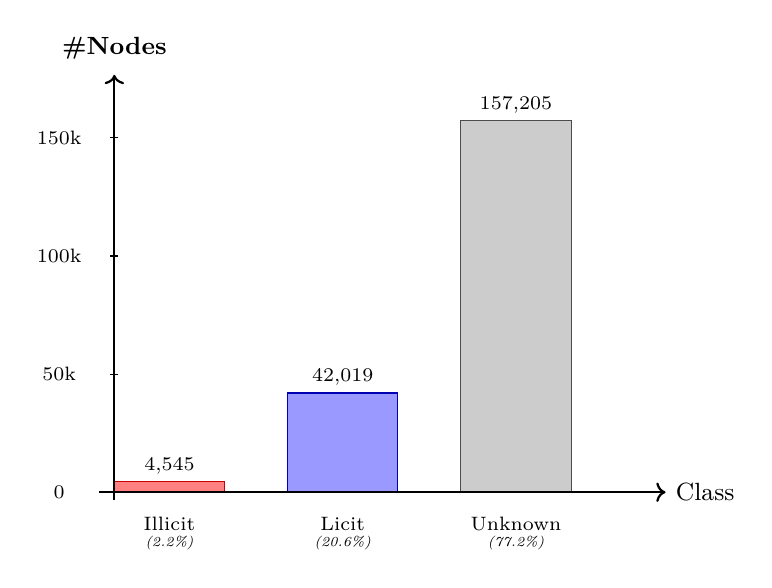
\begin{tikzpicture}[yscale=1.0]
% Bar chart: class distribution (hardcoded bar heights)
% Illicit: 4545 -> 0.137cm; Licit: 42019 -> 1.26cm; Unknown: 157205 -> 4.72cm
% Scale: 1 node = 0.00003 cm (157205 * 0.00003 = 4.72)

% Bars (hardcoded heights)
\fill[red!50!white, draw=red!80!black] (0.0,0) rectangle (1.4, 0.14);
\fill[blue!40!white, draw=blue!70!black] (2.2,0) rectangle (3.6, 1.26);
\fill[gray!40!white, draw=gray!60!black] (4.4,0) rectangle (5.8, 4.72);

% Labels on top of bars
\node at (0.7, 0.34) [font=\scriptsize] {4,545};
\node at (2.9, 1.46) [font=\scriptsize] {42,019};
\node at (5.1, 4.92) [font=\scriptsize] {157,205};

% Percentage labels
\node at (0.7, -0.4) [font=\scriptsize] {Illicit};
\node at (0.7, -0.65) [font=\tiny\itshape] {(2.2\%)};
\node at (2.9, -0.4) [font=\scriptsize] {Licit};
\node at (2.9, -0.65) [font=\tiny\itshape] {(20.6\%)};
\node at (5.1, -0.4) [font=\scriptsize] {Unknown};
\node at (5.1, -0.65) [font=\tiny\itshape] {(77.2\%)};

% Axes
\draw[->, thick] (-0.2, 0) -- (7.0, 0) node[right, font=\small] {Class};
\draw[->, thick] (0, -0.1) -- (0, 5.3) node[above=2pt, font=\small\bfseries] {\#Nodes};

% Y-axis ticks
\draw (0.05,0) -- (-0.05,0); \node at (-0.7,0) [font=\scriptsize] {0};
\draw (0.05,1.5) -- (-0.05,1.5); \node at (-0.7,1.5) [font=\scriptsize] {50k};
\draw (0.05,3.0) -- (-0.05,3.0); \node at (-0.7,3.0) [font=\scriptsize] {100k};
\draw (0.05,4.5) -- (-0.05,4.5); \node at (-0.7,4.5) [font=\scriptsize] {150k};
\end{tikzpicture}
\caption[Class Distribution in Elliptic Dataset]{Class distribution across all 203,769 transaction nodes in the Elliptic Bitcoin Dataset. The illicit class (4,545 nodes, 2.2\%) is severely under-represented relative to the licit (42,019) and unknown (157,205) classes, necessitating class-weighted loss functions.}
\label{fig:class_dist}
\end{figure}

Figure~\ref{fig:temporal_dist} shows the approximate distribution of nodes across the 49 time steps.

\begin{figure}[!htbp]
\centering
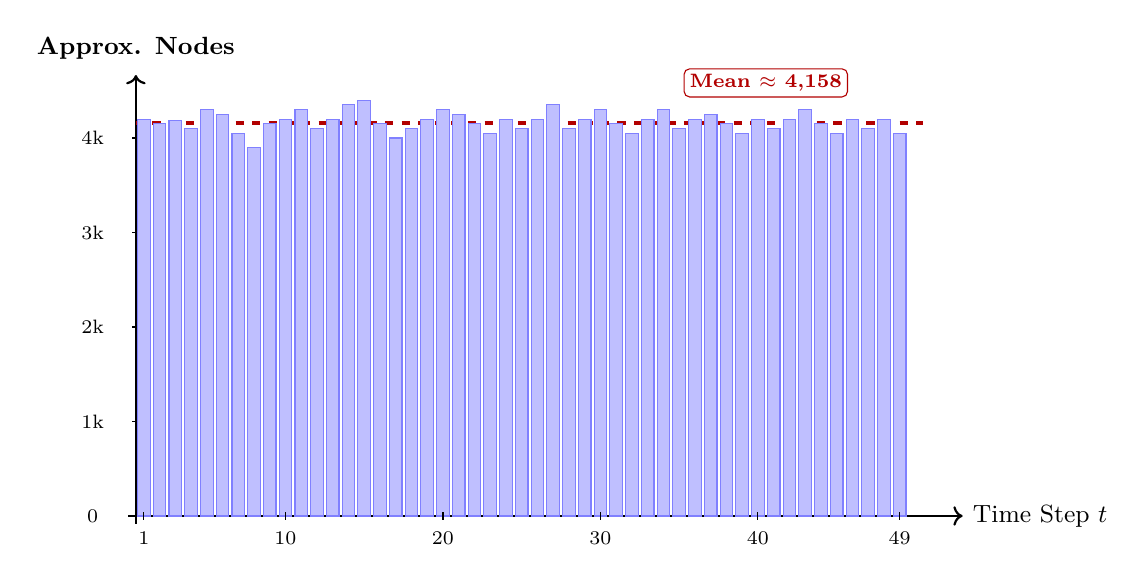
\begin{tikzpicture}
% Temporal distribution: 49 bars at ~4158 average
% Scale: 5000 nodes -> 5.0cm; each bar width = 0.16cm; spacing = 0.20cm total
% Bars represented at unit intervals; each time step bar colour uniform blue

% Axes
\draw[->, thick] (-0.1, 0) -- (10.5, 0) node[right, font=\small] {Time Step $t$};
\draw[->, thick] (0, -0.1) -- (0, 5.6) node[above=2pt, font=\small\bfseries] {Approx. Nodes};

% Y ticks
\draw (0.05,0) -- (-0.05,0); \node[font=\scriptsize] at (-0.55,0) {0};
\draw (0.05,1.2) -- (-0.05,1.2); \node[font=\scriptsize] at (-0.55,1.2) {1k};
\draw (0.05,2.4) -- (-0.05,2.4); \node[font=\scriptsize] at (-0.55,2.4) {2k};
\draw (0.05,3.6) -- (-0.05,3.6); \node[font=\scriptsize] at (-0.55,3.6) {3k};
\draw (0.05,4.8) -- (-0.05,4.8); \node[font=\scriptsize] at (-0.55,4.8) {4k};

% Mean line at 4158 nodes -> 4158/1000 * 1.2 = 4.99
\draw[dashed, ultra thick, red!70!black] (0, 4.99) -- (10.0, 4.99);
\node at (8.0, 5.5) [font=\scriptsize\bfseries, text=red!70!black, fill=white, draw=red!70!black, rounded corners=2pt, inner sep=2pt] {Mean $\approx$ 4,158};

% 49 bars, each 0.18cm wide, spaced 0.20cm apart, heights ~5cm (varying slightly)
% Heights in cm (representing ~4000-4400 nodes, scale: 1k nodes = 1.2cm)
\foreach \i/\hi in {
  1/5.04, 2/4.98, 3/5.02, 4/4.92, 5/5.16, 6/5.10, 7/4.86, 8/4.68,
  9/4.98, 10/5.04, 11/5.16, 12/4.92, 13/5.04, 14/5.22, 15/5.28, 16/4.98,
  17/4.80, 18/4.92, 19/5.04, 20/5.16, 21/5.10, 22/4.98, 23/4.86, 24/5.04,
  25/4.92, 26/5.04, 27/5.22, 28/4.92, 29/5.04, 30/5.16, 31/4.98, 32/4.86,
  33/5.04, 34/5.16, 35/4.92, 36/5.04, 37/5.10, 38/4.98, 39/4.86, 40/5.04,
  41/4.92, 42/5.04, 43/5.16, 44/4.98, 45/4.86, 46/5.04, 47/4.92, 48/5.04, 49/4.86
}{
  \pgfmathsetmacro\xpos{(\i-1)*0.20 + 0.10}
  \fill[blue!25, draw=blue!50] (\xpos-0.08, 0) rectangle (\xpos+0.08, \hi);
}

% X ticks
\foreach \t/\xpos in {1/0.10, 10/1.90, 20/3.90, 30/5.90, 40/7.90, 49/9.70}{
  \draw (\xpos, 0.05) -- (\xpos, -0.05);
  \node[font=\scriptsize] at (\xpos, -0.28) {\t};
}
\end{tikzpicture}
\caption[Temporal Distribution of Transactions]{Approximate distribution of transaction nodes across the 49 time steps of the Elliptic Bitcoin Dataset. The red dashed line indicates the mean of approximately 4,158 nodes per time step. Values are representative approximations; exact per-step counts require computation from the raw dataset.}
\label{fig:temporal_dist}
\end{figure}


---

\section{Algorithm and Model Design}
\label{sec:algo_design}

\subsection{Objective 1 — Temporal Graph Construction}
\label{subsec:graph_construction}

Figure~\ref{fig:graph_construction} illustrates the temporal graph construction workflow.

\begin{figure}[!htbp]
\centering
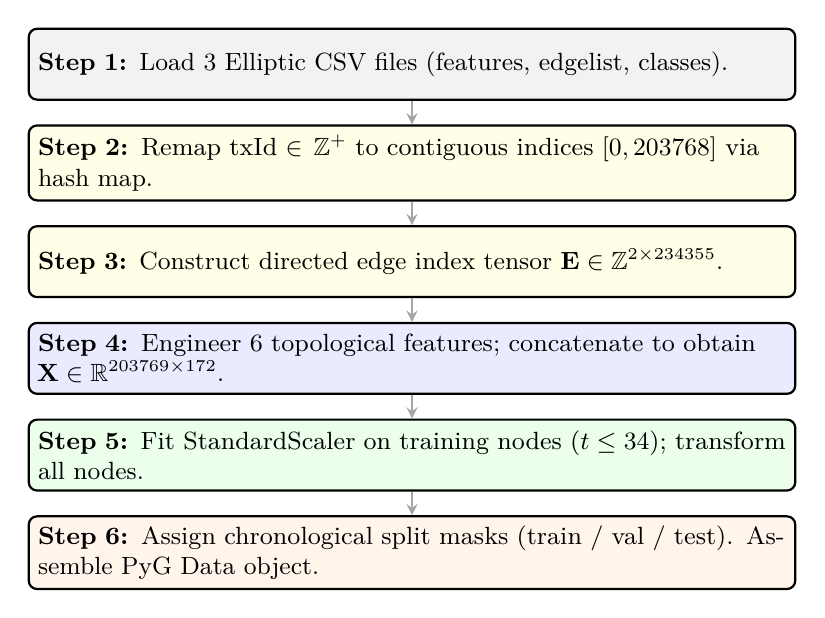
\begin{tikzpicture}[
    flowstep/.style={rectangle, draw=black, fill=yellow!10, rounded corners=3pt, thick,
                 text width=9.5cm, minimum height=0.9cm, align=left, font=\small},
    arrow/.style={->, >=stealth, thick, draw=gray!70},
]
\node[flowstep, fill=gray!10] (s1)
  {\textbf{Step 1:} Load 3 Elliptic CSV files (features, edgelist, classes).};
\node[flowstep, below=0.3cm of s1, fill=yellow!10] (s2)
  {\textbf{Step 2:} Remap txId $\in \mathbb{Z}^+$ to contiguous indices $[0, 203768]$ via hash map.};
\node[flowstep, below=0.3cm of s2] (s3)
  {\textbf{Step 3:} Construct directed edge index tensor $\mathbf{E} \in \mathbb{Z}^{2 \times 234355}$.};
\node[flowstep, below=0.3cm of s3, fill=blue!8] (s4)
  {\textbf{Step 4:} Engineer 6 topological features; concatenate to obtain $\mathbf{X} \in \mathbb{R}^{203769 \times 172}$.};
\node[flowstep, below=0.3cm of s4, fill=green!8] (s5)
  {\textbf{Step 5:} Fit StandardScaler on training nodes ($t \leq 34$); transform all nodes.};
\node[flowstep, below=0.3cm of s5, fill=orange!8] (s6)
  {\textbf{Step 6:} Assign chronological split masks (train / val / test). Assemble PyG Data object.};

\draw[arrow] (s1) -- (s2);
\draw[arrow] (s2) -- (s3);
\draw[arrow] (s3) -- (s4);
\draw[arrow] (s4) -- (s5);
\draw[arrow] (s5) -- (s6);
\end{tikzpicture}
\caption[Temporal Graph Construction Workflow]{Step-by-step workflow for constructing the temporal graph from the Elliptic Bitcoin Dataset.}
\label{fig:graph_construction}
\end{figure}

\noindent \textbf{Engineered Topological Features:} In addition to the raw 166 dataset features, six domain-specific topological features are engineered to provide immediate structural signals relevant to AML. Table~\ref{tab:engineered_features} defines each feature.

\begin{table}[!htbp]
\centering
\caption[Engineered Topological Features]{Six engineered topological features appended to each transaction node, expanding the feature dimension from 166 to 172.}
\label{tab:engineered_features}
\begin{tabularx}{\textwidth}{>{\hsize=0.85\hsize}L >{\hsize=1.0\hsize}L >{\hsize=1.15\hsize}L}
\toprule
\textbf{Feature} & \textbf{Mathematical Definition} & \textbf{AML Rationale} \\
\midrule
Out-Degree ($d_{\text{out}}$) & $\sum_{(v, u) \in E} 1$ & Identifies fund-dispersal nodes (smurfing originators). \\
In-Degree ($d_{\text{in}}$) & $\sum_{(u, v) \in E} 1$ & Identifies fund-aggregation nodes (smurfing collection points). \\
Fan-Out Ratio & $\dfrac{d_{\text{out}}}{d_{\text{in}} + d_{\text{out}} + \epsilon}$ & High ratio ($> 0.8$) signifies fund dispersal phase. \\
Fan-In Ratio & $\dfrac{d_{\text{in}}}{d_{\text{in}} + d_{\text{out}} + \epsilon}$ & High ratio ($> 0.8$) signifies fund aggregation phase. \\
Temporal Recency & $t_v / 49.0$ & Continuous temporal position of transaction in $[0, 1]$. \\
Neighbour Time Delta & $\frac{1}{|\mathcal{N}(v)|} \sum_{u \in \mathcal{N}(v)} |t_v - t_u|$ & Measures transaction velocity and dormancy duration. \\
\bottomrule
\end{tabularx}
\end{table}

\noindent \textbf{Mathematical Formulation:}
\begin{equation}
\mathbf{X}^{(172)} = \left[ \mathbf{X}^{(166)}_{\text{raw}} \;\big\|\; d_{\text{out}}, \; d_{\text{in}}, \; r_{\text{out}}, \; r_{\text{in}}, \; \frac{t_v}{49}, \; \bar{\delta}_{\mathcal{N}(v)} \right]
\label{eq:feature_expansion}
\end{equation}

Figure~\ref{fig:graph_representation} illustrates the temporal graph with nodes, directed edges, and time step labels.

\begin{figure}[!htbp]
\centering
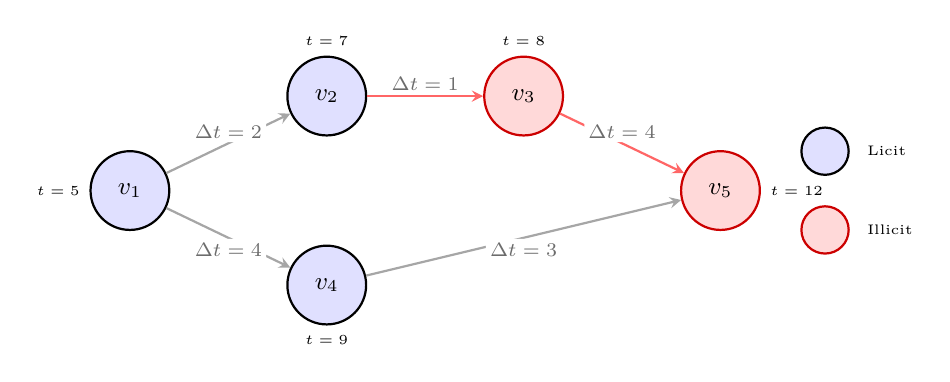
\begin{tikzpicture}[
    tnode/.style={circle, draw=black, fill=blue!12, thick, minimum size=1.0cm, font=\small},
    inode/.style={circle, draw=red!80!black, fill=red!15, thick, minimum size=1.0cm, font=\small},
    edge/.style={->, >=stealth, thick, draw=gray!70},
    iedge/.style={->, >=stealth, thick, draw=red!60},
    tlabel/.style={font=\scriptsize, text=gray!85!black, fill=white, inner sep=1.5pt, rounded corners=1pt},
]
\node[tnode, label=left:{\tiny $t=5$}] (n1) at (0, 0) {$v_1$};
\node[tnode, label=above:{\tiny $t=7$}] (n2) at (2.5, 1.2) {$v_2$};
\node[inode, label=above:{\tiny $t=8$}] (n3) at (5.0, 1.2) {$v_3$};
\node[tnode, label=below:{\tiny $t=9$}] (n4) at (2.5,-1.2) {$v_4$};
\node[inode, label=right:{\tiny $t=12$}] (n5) at (7.5, 0) {$v_5$};

\draw[edge] (n1) -- (n2) node[midway, above, tlabel] {$\Delta t=2$};
\draw[edge] (n1) -- (n4) node[midway, below, tlabel] {$\Delta t=4$};
\draw[iedge] (n2) -- (n3) node[midway, above, tlabel] {$\Delta t=1$};
\draw[iedge] (n3) -- (n5) node[midway, above, tlabel] {$\Delta t=4$};
\draw[edge] (n4) -- (n5) node[midway, below, tlabel] {$\Delta t=3$};

% Legend
\node[tnode, minimum size=0.6cm, right=0.5cm of n5, yshift=0.5cm] (ll) {};
\node[right=0.1cm of ll, font=\tiny] {Licit};
\node[inode, minimum size=0.6cm, right=0.5cm of n5, yshift=-0.5cm] (li) {};
\node[right=0.1cm of li, font=\tiny] {Illicit};
\end{tikzpicture}
\caption[Temporal Graph Representation]{Illustration of the temporal graph $G = (V, E, \mathbf{X}, \mathbf{T})$. Each node $v_i$ is labelled with its time step $t$. Directed edges show UTXO fund flows, with $\Delta t$ labels indicating the time difference between connected transactions. Blue nodes are licit; red nodes are illicit.}
\label{fig:graph_representation}
\end{figure}

\subsection{Objective 2 — Learnable Fourier Time Encoding}
\label{subsec:fourier_encoding}

This subsection describes the core technical novelty of TemporalAML: a trainable Fourier time encoding module integrated directly into the graph attention mechanism.

\vspace{0.5em}
\noindent \textbf{Motivation:} Standard TGAT~\cite{xu2020tgat} uses fixed sinusoidal frequencies calibrated for NLP token sequences:
\begin{equation}
\omega_k^{\text{fixed}} = 10000^{-2k/d}, \quad k = 1, 2, \ldots, d/2
\label{eq:fixed_freq}
\end{equation}
Cryptocurrency transaction intervals are non-stationary and bursty (following a power-law distribution). Fixed frequencies cannot adapt to the specific time scales of rapid layering hops (minutes) or slow dormancy cycles (weeks). TemporalAML replaces fixed frequencies with \textbf{trainable parameters learned by gradient descent}.

\vspace{0.5em}
\noindent \textbf{Theoretical Foundation:} By Bochner's Theorem~\cite{bochner1933monotone}, any continuous, shift-invariant kernel $K(\Delta t) = \psi(t_i - t_j)$ can be expressed as the Fourier transform of a positive measure. This justifies representing temporal similarity through a sum of complex exponentials (equivalently, sin/cos pairs).

\vspace{0.5em}
\noindent \textbf{Learnable Fourier Time Encoding Formula:}
\begin{equation}
\Phi(\Delta t) = \sqrt{\frac{1}{k}} \Big[ \cos(\omega_1 \Delta t + \phi_1), \; \sin(\omega_1 \Delta t + \phi_1), \; \ldots, \; \cos(\omega_k \Delta t + \phi_k), \; \sin(\omega_k \Delta t + \phi_k) \Big]
\label{eq:fourier_encoding}
\end{equation}
where:
\begin{itemize}
	\item $\Delta t = t_{\text{target}} - t_{\text{source}} \geq 0$ is the continuous edge time delta.
	\item $k = 64$ is the number of frequency components; the output dimension is $d_t = 2k = 128$.
	\item $\boldsymbol{\omega} \in \mathbb{R}^{k}$ are \textbf{learnable frequency parameters}, initialised from $\mathcal{N}(0, 0.01)$.
	\item $\boldsymbol{\phi} \in \mathbb{R}^{k}$ are \textbf{learnable phase shift parameters}, initialised to zero.
	\item $\sqrt{1/k}$ is a normalisation scalar.
\end{itemize}

\vspace{0.5em}
\noindent \textbf{Learnability via Gradient Descent:} The gradient of the encoding with respect to frequency parameter $\omega_j$ is:
\begin{equation}
\frac{\partial \Phi_j(\Delta t)}{\partial \omega_j} = -\Delta t \cdot \sin(\omega_j \Delta t + \phi_j) \neq 0
\label{eq:fourier_gradient}
\end{equation}
Since this gradient is non-zero for almost all $\Delta t > 0$, the loss gradient $\frac{\partial \mathcal{L}}{\partial \boldsymbol{\omega}} = \frac{\partial \mathcal{L}}{\partial \Phi} \cdot \frac{\partial \Phi}{\partial \boldsymbol{\omega}}$ flows back to dynamically calibrate frequencies to the characteristic velocity of cryptocurrency laundering hops.

Figure~\ref{fig:fourier_arch} shows the Fourier Time Encoding architecture.

\begin{figure}[!htbp]
\centering
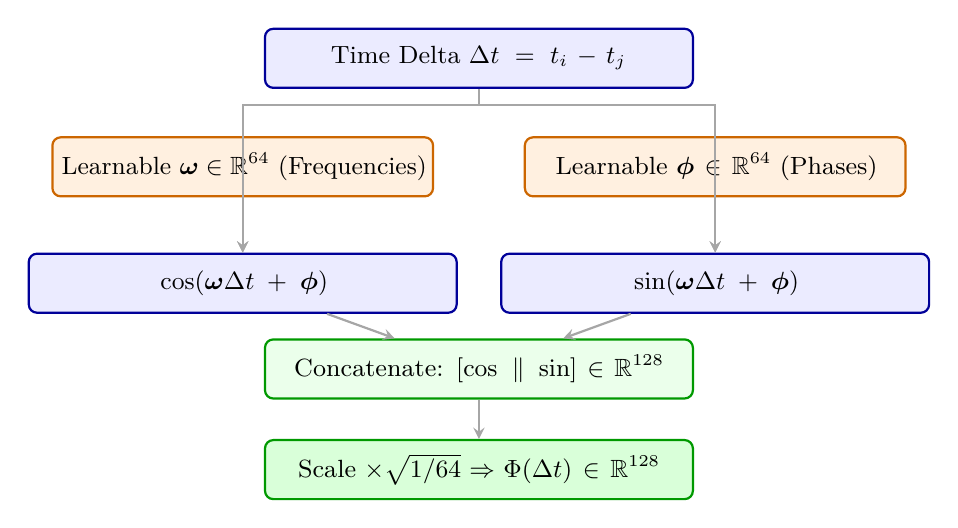
\begin{tikzpicture}[
    block/.style={rectangle, draw=blue!60!black, fill=blue!8, rounded corners=3pt, thick,
                  text width=5.2cm, minimum height=0.75cm, align=center, font=\small},
    param/.style={rectangle, draw=orange!80!black, fill=orange!12, rounded corners=3pt, thick,
                  text width=4.6cm, minimum height=0.75cm, align=center, font=\small},
    arrow/.style={->, >=stealth, thick, draw=gray!70},
    concat/.style={rectangle, draw=green!60!black, fill=green!8, rounded corners=3pt, thick,
                   text width=5.2cm, minimum height=0.75cm, align=center, font=\small},
]
\node[block] (dt) {Time Delta $\Delta t = t_i - t_j$};
\node[param, below=0.6cm of dt, xshift=-3.0cm] (omega) {Learnable $\boldsymbol{\omega} \in \mathbb{R}^{64}$ (Frequencies)};
\node[param, below=0.6cm of dt, xshift=3.0cm] (phi) {Learnable $\boldsymbol{\phi} \in \mathbb{R}^{64}$ (Phases)};
\node[block, below=0.7cm of omega] (cos) {$\cos(\boldsymbol{\omega}\Delta t + \boldsymbol{\phi})$};
\node[block, below=0.7cm of phi] (sin) {$\sin(\boldsymbol{\omega}\Delta t + \boldsymbol{\phi})$};
\node[concat, below=0.7cm of $(cos)!0.5!(sin)$] (cat) {Concatenate: $[\cos \;\|\; \sin] \in \mathbb{R}^{128}$};
\node[block, below=0.5cm of cat, fill=green!15, draw=green!60!black] (norm) {Scale $\times \sqrt{1/64}$ $\Rightarrow$ $\Phi(\Delta t) \in \mathbb{R}^{128}$};

\draw[arrow] (dt.south) -- ++(0,-0.2) -| (cos.north);
\draw[arrow] (dt.south) -- ++(0,-0.2) -| (sin.north);
\draw[arrow] (omega) -- (cos);
\draw[arrow] (phi) -- (sin);
\draw[arrow] (cos) -- (cat);
\draw[arrow] (sin) -- (cat);
\draw[arrow] (cat) -- (norm);
\end{tikzpicture}
\caption[Learnable Fourier Time Encoding Architecture]{Architecture of the Learnable Fourier Time Encoding module. The time delta $\Delta t$ is multiplied with trainable frequency parameters $\boldsymbol{\omega}$ and summed with trainable phase shifts $\boldsymbol{\phi}$, projected through cosine and sine functions, concatenated, and normalised to produce a 128-dimensional temporal embedding $\Phi(\Delta t)$.}
\label{fig:fourier_arch}
\end{figure}

\subsection{Objective 3 — Temporal Graph Attention Network (TGAT)}
\label{subsec:tgat}

\subsubsection{Temporal Neighbourhood and Causal Masking}

For each target node $v_i$ with time step $t_i$, the causal temporal neighbourhood is defined as:
\begin{equation}
\mathcal{N}_{\text{causal}}(v_i) = \{ v_j \in \mathcal{N}(v_i) \mid t_j \leq t_i \}
\label{eq:causal_neighborhood}
\end{equation}
This ensures that the attention mechanism only aggregates information from transactions occurring \textit{at or before} the target transaction, preventing future data leakage during both training and inference.

\subsubsection{TGAT Layer Computation}

Each TGATConv layer computes temporally-aware node representations through a query-key-value attention mechanism. Let $\mathbf{h}_i^{(l)}$ denote the node $i$ representation at layer $l$:

\begin{equation}
\mathbf{q}_i = \left[\mathbf{h}_i^{(l)} \;\big\|\; \Phi(0)\right] \mathbf{W}_Q
\label{eq:query}
\end{equation}

\begin{equation}
\mathbf{k}_j = \left[\mathbf{h}_j^{(l)} \;\big\|\; \Phi(t_i - t_j)\right] \mathbf{W}_K, \qquad \mathbf{v}_j = \left[\mathbf{h}_j^{(l)} \;\big\|\; \Phi(t_i - t_j)\right] \mathbf{W}_V
\label{eq:key_value}
\end{equation}

\begin{equation}
\alpha_{ij} = \text{softmax}\left( \frac{\mathbf{q}_i \mathbf{k}_j^\top}{\sqrt{d_k}} \right) = \frac{\exp\!\left( \frac{\mathbf{q}_i \mathbf{k}_j^\top}{\sqrt{d_k}} \right)}{\sum_{u \in \mathcal{N}_{\text{causal}}(i)} \exp\!\left( \frac{\mathbf{q}_i \mathbf{k}_u^\top}{\sqrt{d_k}} \right)}
\label{eq:attention}
\end{equation}

\begin{equation}
\mathbf{h}_i^{(l+1)} = \text{LayerNorm}\!\left( \sum_{j \in \mathcal{N}_{\text{causal}}(i)} \alpha_{ij} \mathbf{v}_j \;+\; \mathbf{W}_{\text{res}} \mathbf{h}_i^{(l)} \right)
\label{eq:tgat_update}
\end{equation}

\noindent where $\mathbf{W}_Q, \mathbf{W}_K, \mathbf{W}_V \in \mathbb{R}^{(d_h + d_t) \times d_k}$ are learnable projection matrices, $d_h = 128$ is the node embedding dimension, $d_t = 128$ is the Fourier encoding dimension, $d_k = 64$ is the attention head dimension, and $\mathbf{W}_{\text{res}}$ is the residual projection matrix.

Figure~\ref{fig:tgat_arch} illustrates the complete TGAT layer architecture.

\begin{figure}[!htbp]
\centering
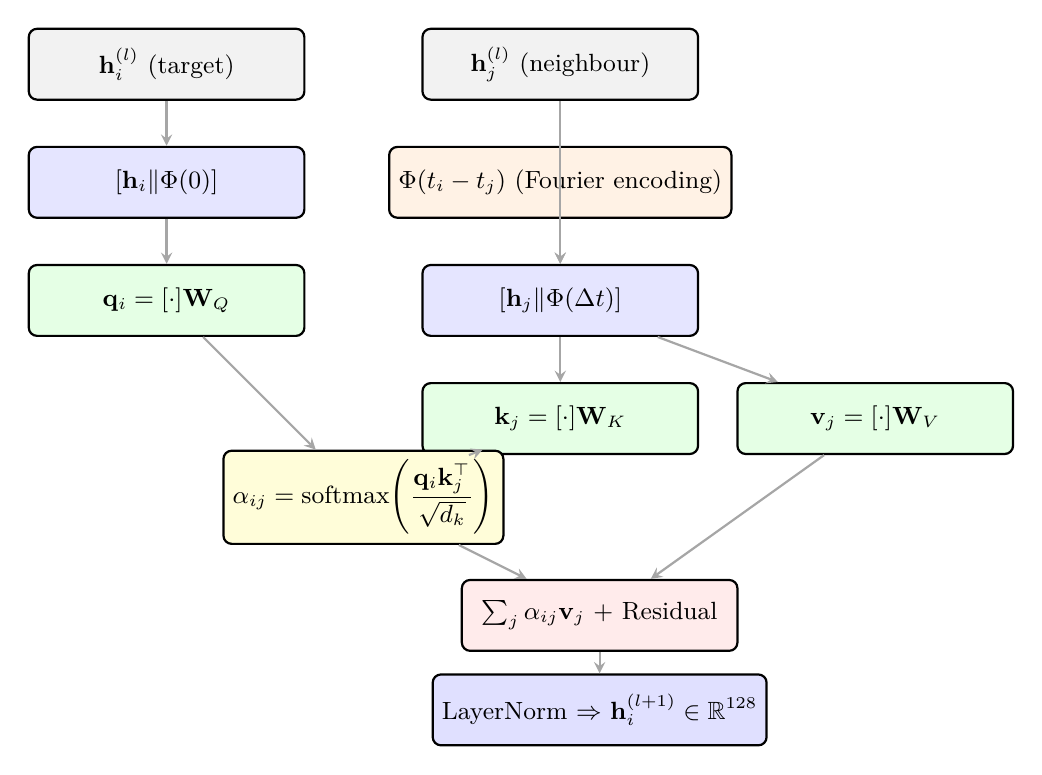
\begin{tikzpicture}[
    block/.style={rectangle, draw=black, fill=blue!8, rounded corners=3pt, thick,
                  minimum width=3.5cm, minimum height=0.9cm, align=center, font=\small},
    arrow/.style={->, >=stealth, thick, draw=gray!70},
    label/.style={font=\scriptsize\itshape, text=gray!70},
]
% Input row
\node[block, fill=gray!10] (xi) at (0,0) {$\mathbf{h}_i^{(l)}$ (target)};
\node[block, fill=gray!10] (xj) at (5,0) {$\mathbf{h}_j^{(l)}$ (neighbour)};
\node[block, fill=orange!10] (phi) at (5,-1.5) {$\Phi(t_i - t_j)$ (Fourier encoding)};

% Concat
\node[block, fill=blue!10] (concatq) at (0,-1.5) {$[\mathbf{h}_i \| \Phi(0)]$};
\node[block, fill=blue!10] (concatk) at (5,-3.0) {$[\mathbf{h}_j \| \Phi(\Delta t)]$};

% QKV
\node[block, fill=green!10] (q) at (0,-3.0) {$\mathbf{q}_i = [\cdot]\mathbf{W}_Q$};
\node[block, fill=green!10] (k) at (5,-4.5) {$\mathbf{k}_j = [\cdot]\mathbf{W}_K$};
\node[block, fill=green!10] (v) at (9,-4.5) {$\mathbf{v}_j = [\cdot]\mathbf{W}_V$};

% Attention
\node[block, fill=yellow!15] (attn) at (2.5,-5.5) {$\alpha_{ij} = \text{softmax}\!\left(\dfrac{\mathbf{q}_i\mathbf{k}_j^\top}{\sqrt{d_k}}\right)$};

% Aggregation
\node[block, fill=red!8] (agg) at (5.5,-7.0) {$\sum_{j} \alpha_{ij}\mathbf{v}_j$ + Residual};
\node[block, fill=blue!12] (out) at (5.5,-8.2) {LayerNorm $\Rightarrow$ $\mathbf{h}_i^{(l+1)} \in \mathbb{R}^{128}$};

% Arrows
\draw[arrow] (xi) -- (concatq);
\draw[arrow] (concatq) -- (q);
\draw[arrow] (xj) -- (concatk);
\draw[arrow] (phi) -- (concatk);
\draw[arrow] (concatk) -- (k);
\draw[arrow] (concatk) -- (v);
\draw[arrow] (q) -- (attn);
\draw[arrow] (k) -- (attn);
\draw[arrow] (attn) -- (agg);
\draw[arrow] (v) -- (agg);
\draw[arrow] (agg) -- (out);
\end{tikzpicture}
\caption[TGAT Layer Architecture]{Architecture of a single Temporal Graph Attention (TGAT) layer. The target node $v_i$ and each causal neighbour $v_j$ are concatenated with their respective Fourier time encodings ($\Phi(0)$ for the target and $\Phi(t_i - t_j)$ for the neighbour) before attention projection. The attention coefficient $\alpha_{ij}$ modulates the aggregation of neighbour value vectors, with a residual connection and layer normalisation.}
\label{fig:tgat_arch}
\end{figure}

\subsubsection{Multi-Pattern AML Detection Heads}
\label{subsubsec:pattern_heads}

The two-layer TGATConv encoder produces a shared 128-dimensional latent embedding $\mathbf{Z} \in \mathbb{R}^{N \times 128}$ for all nodes. Three parallel feed-forward classification heads operate on these shared embeddings:

\begin{align}
\hat{y}^{\text{circ}}_v &= \sigma\!\left( \mathbf{W}^{\text{circ}}_2 \;\text{ReLU}\!\left(\mathbf{W}^{\text{circ}}_1 \mathbf{z}_v + \mathbf{b}^{\text{circ}}_1\right) + \mathbf{b}^{\text{circ}}_2 \right) \label{eq:circ_head} \\
\hat{y}^{\text{lay}}_v &= \sigma\!\left( \mathbf{W}^{\text{lay}}_2 \;\text{ReLU}\!\left(\mathbf{W}^{\text{lay}}_1 \mathbf{z}_v + \mathbf{b}^{\text{lay}}_1\right) + \mathbf{b}^{\text{lay}}_2 \right) \label{eq:lay_head} \\
\hat{y}^{\text{smurf}}_v &= \sigma\!\left( \mathbf{W}^{\text{smurf}}_2 \;\text{ReLU}\!\left(\mathbf{W}^{\text{smurf}}_1 \mathbf{z}_v + \mathbf{b}^{\text{smurf}}_1\right) + \mathbf{b}^{\text{smurf}}_2 \right) \label{eq:smurf_head}
\end{align}

where $\sigma$ denotes the sigmoid activation function and $\mathbf{z}_v \in \mathbb{R}^{128}$ is the shared TGAT node embedding.

\vspace{0.5em}
\noindent \textbf{Joint Multi-Task Loss:}
\begin{equation}
\begin{split}
\mathcal{L}_{\text{total}} = {} & \lambda_1 \;\text{WBCE}(\hat{y}^{\text{circ}}, y^{\text{circ}}, w_1) + \lambda_2 \;\text{WBCE}(\hat{y}^{\text{lay}}, y^{\text{lay}}, w_2) \\
& + \lambda_3 \;\text{WBCE}(\hat{y}^{\text{smurf}}, y^{\text{smurf}}, w_3)
\end{split}
\label{eq:joint_loss}
\end{equation}
where $\text{WBCE}$ is the Weighted Binary Cross-Entropy loss, $w_k = N_{\text{neg},k} / N_{\text{pos},k}$ is the positive-class weight for pattern $k$ to mitigate class imbalance, and $\lambda_1 = \lambda_2 = \lambda_3 = 1.0$.

\vspace{0.5em}
\noindent \textbf{Ground-Truth Pattern Label Mining:} Because the Elliptic dataset provides only binary illicit/licit labels, pattern-specific ground-truth labels are mined algorithmically from the graph topology:
\begin{itemize}
	\item $y^{\text{circ}} = 1$ for illicit nodes participating in a Strongly Connected Component (SCC) of size $\geq 2$, computed using Tarjan's SCC algorithm.
	\item $y^{\text{lay}} = 1$ for illicit nodes on directed paths of length $\geq 3$ with monotonically increasing timestamps ($t_{k+1} \geq t_k$), identified by temporal directed BFS.
	\item $y^{\text{smurf}} = 1$ for illicit nodes with out-degree $d_{\text{out}} \geq 10$ or in-degree $d_{\text{in}} \geq 10$.
\end{itemize}

\noindent \textbf{Domain Constraint Note:} The Bitcoin UTXO model is a strict Directed Acyclic Graph at the transaction level—transaction outputs cannot be consumed by ancestor transactions. Consequently, closed transaction-level cycles ($A \to B \to C \to A$) cannot exist in the raw Elliptic transaction graph. Circular transfer detection is therefore architecturally included for completeness and future applicability to wallet-entity-level graphs, while the primary pattern signals in the current framework are Layering Chains and Smurfing.

\vspace{1em}
\noindent Figures~\ref{fig:circular_pattern}, \ref{fig:layering_pattern}, and \ref{fig:smurfing_pattern} illustrate the three targeted laundering patterns.

\begin{figure}[!htbp]
\centering
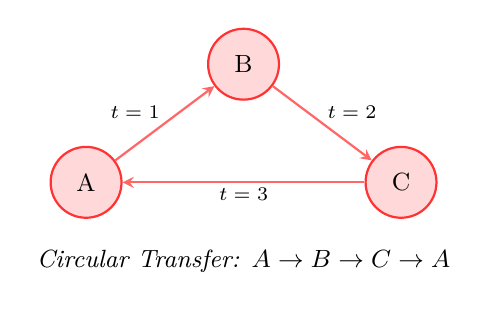
\begin{tikzpicture}[
    wnode/.style={circle, draw=red!80, fill=red!15, thick, minimum size=0.9cm, font=\small},
    edge/.style={->, >=stealth, thick, draw=red!60},
]
\node[wnode] (A) at (0,0) {A};
\node[wnode] (B) at (2,1.5) {B};
\node[wnode] (C) at (4,0) {C};
\draw[edge] (A) -- (B) node[midway, above left, font=\scriptsize, fill=white, inner sep=1.5pt, rounded corners=1pt] {$t=1$};
\draw[edge] (B) -- (C) node[midway, above right, font=\scriptsize, fill=white, inner sep=1.5pt, rounded corners=1pt] {$t=2$};
\draw[edge] (C) -- (A) node[midway, below, font=\scriptsize, fill=white, inner sep=1.5pt, rounded corners=1pt] {$t=3$};
\node at (2, -1.0) [font=\small\itshape] {Circular Transfer: $A \to B \to C \to A$};
\end{tikzpicture}
\caption[Circular Transfer Pattern]{Circular Transfer pattern: funds cycle through a closed loop ($A \to B \to C \to A$) to simulate wash trading, confuse audit tracing systems, and obscure the origin of illicit proceeds. Detected via Tarjan's Strongly Connected Components algorithm.}
\label{fig:circular_pattern}
\end{figure}

\begin{figure}[!htbp]
\centering
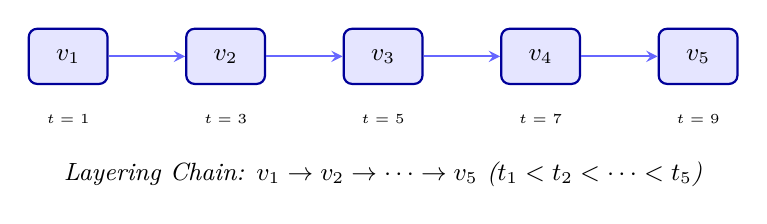
\begin{tikzpicture}[
    wnode/.style={rectangle, draw=blue!60!black, fill=blue!10, thick, rounded corners=3pt, minimum width=1.0cm, minimum height=0.7cm, font=\small},
    edge/.style={->, >=stealth, thick, draw=blue!60},
]
\node[wnode] (n1) at (0,0) {$v_1$};
\node[wnode] (n2) at (2,0) {$v_2$};
\node[wnode] (n3) at (4,0) {$v_3$};
\node[wnode] (n4) at (6,0) {$v_4$};
\node[wnode] (n5) at (8,0) {$v_5$};
\node at (0,-0.8) [font=\tiny\itshape] {$t=1$};
\node at (2,-0.8) [font=\tiny\itshape] {$t=3$};
\node at (4,-0.8) [font=\tiny\itshape] {$t=5$};
\node at (6,-0.8) [font=\tiny\itshape] {$t=7$};
\node at (8,-0.8) [font=\tiny\itshape] {$t=9$};
\draw[edge] (n1) -- (n2);
\draw[edge] (n2) -- (n3);
\draw[edge] (n3) -- (n4);
\draw[edge] (n4) -- (n5);
\node at (4,-1.5) [font=\small\itshape] {Layering Chain: $v_1 \to v_2 \to \cdots \to v_5$ ($t_1 < t_2 < \cdots < t_5$)};
\end{tikzpicture}
\caption[Layering Chain Pattern]{Layering Chain pattern: funds are forwarded across a linear sequence of transaction hops with monotonically increasing timestamps ($t_1 < t_2 < \ldots < t_k$, $k \geq 3$). Rapid layering exploits hop-decay AML heuristics. Detected via temporal directed BFS.}
\label{fig:layering_pattern}
\end{figure}

\begin{figure}[!htbp]
\centering
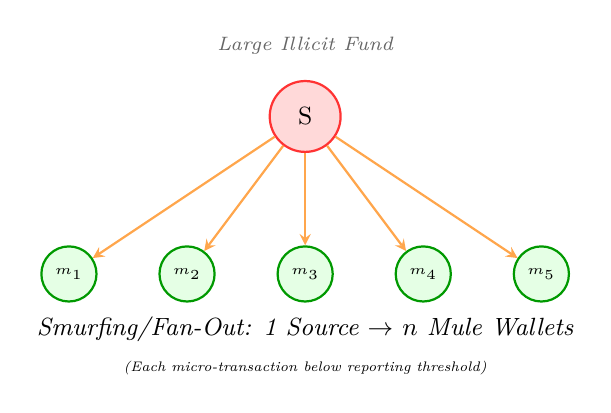
\begin{tikzpicture}[
    source/.style={circle, draw=red!80, fill=red!15, thick, minimum size=0.9cm, font=\small},
    mule/.style={circle, draw=green!60!black, fill=green!10, thick, minimum size=0.7cm, font=\tiny},
    edge/.style={->, >=stealth, thick, draw=orange!70},
]
\node[source] (S) at (3,0) {S};
\node[mule] (m1) at (0,-2) {$m_1$};
\node[mule] (m2) at (1.5,-2) {$m_2$};
\node[mule] (m3) at (3,-2) {$m_3$};
\node[mule] (m4) at (4.5,-2) {$m_4$};
\node[mule] (m5) at (6,-2) {$m_5$};
\draw[edge] (S) -- (m1);
\draw[edge] (S) -- (m2);
\draw[edge] (S) -- (m3);
\draw[edge] (S) -- (m4);
\draw[edge] (S) -- (m5);
\node at (3, 0.9) [font=\scriptsize\itshape, text=gray!80!black] {Large Illicit Fund};
\node at (3,-2.7) [font=\small\itshape] {Smurfing/Fan-Out: 1 Source $\to$ $n$ Mule Wallets};
\node at (3,-3.2) [font=\tiny\itshape] {(Each micro-transaction below reporting threshold)};
\end{tikzpicture}
\caption[Smurfing / Fan-Out Pattern]{Smurfing (Fan-Out / Structuring) pattern: a single source transaction splits a large illicit fund into multiple micro-transactions directed to many destination mule wallets, each below mandatory reporting thresholds (e.g., \$10,000 FATF limit). Detected by degree thresholding ($d_{\text{out}} \geq 10$).}
\label{fig:smurfing_pattern}
\end{figure}

\subsection{Objective 4 — Per-Pattern Subgraph Explainability}
\label{subsec:explainability}

\subsubsection{Why Explainability is Necessary in AML}

Financial regulators (FATF, FinCEN, FCA) require AML alerts to be accompanied by auditable evidence trails sufficient to support Suspicious Activity Report (SAR) filing. A scalar probability score alone is not actionable: compliance officers need to know \textit{which specific transactions} formed the suspicious pattern and \textit{in what temporal order} funds flowed through the network.

\subsubsection{GNNExplainer}

GNNExplainer~\cite{ying2019gnnexplainer} is a model-agnostic post-hoc explainability method that, given a trained GNN and a target node $v^*$, learns a soft edge mask $\mathbf{M} \in [0,1]^{|E_{s}|}$ by solving the following mutual information maximisation problem:
\begin{equation}
\max_{\mathbf{M}} \; \text{MI}\!\left( Y_{v^*}^G, \; Y_{v^*}^{G_s} \right) = H\!\left(Y_{v^*}^G\right) - H\!\left(Y_{v^*}^G \mid G_s = (A \odot \sigma(\mathbf{M}), \mathbf{X})\right)
\label{eq:gnnexplainer}
\end{equation}
where $Y_{v^*}^G$ is the model's prediction on the full graph, $G_s$ is the masked subgraph, $\odot$ is element-wise multiplication, and $H(\cdot)$ is the Shannon entropy. The optimisation is performed by gradient ascent on $\mathbf{M}$ for a fixed number of epochs (typically 200), after which a threshold is applied to select the top-$k$ most important edges.

\subsubsection{Per-Pattern Evidence Generation}

For each flagged alert node $v^*$:
\begin{enumerate}
	\item GNNExplainer is activated independently for each positive pattern head (e.g., if $\hat{y}^{\text{lay}}_{v^*} > 0.5$, the layering head's prediction is explained).
	\item The optimised edge mask $\mathbf{M}^*$ identifies the $k$ most important transaction edges contributing to the pattern classification.
	\item These edges, along with their associated nodes and timestamps, are extracted to form the \textit{evidence subgraph} $G_s$.
	\item The evidence subgraph nodes are sorted by timestamp to generate a \textit{time-ordered transaction chain}.
\end{enumerate}

Figure~\ref{fig:gnnexplainer_workflow} illustrates the GNNExplainer workflow.

\begin{figure}[!htbp]
\centering
\vspace{-0.5em}
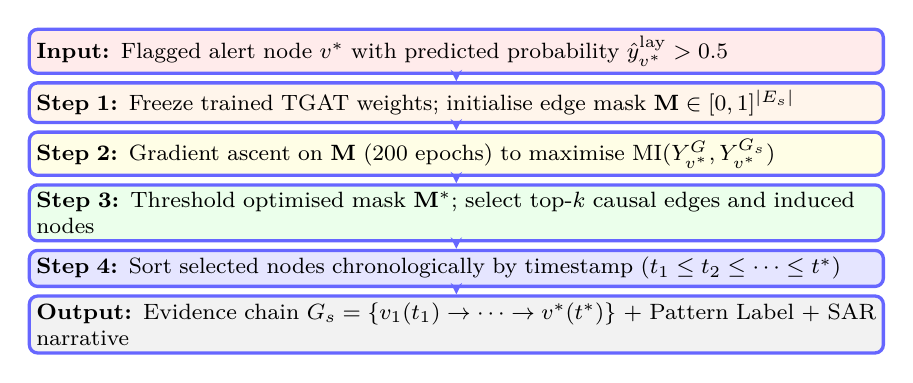
\begin{tikzpicture}[
  block/.style={rectangle, draw=blue!60, fill=blue!5, very thick,
    text width=0.88\textwidth, align=left, rounded corners=3pt,
    font=\footnotesize, inner sep=2.5pt},
  arrow/.style={->, >=stealth, thick, color=blue!60}
]
\node[block, fill=red!8] (input)
  {\textbf{Input:} Flagged alert node $v^*$ with predicted probability $\hat{y}^{\text{lay}}_{v^*} > 0.5$};
\node[block, below=0.08cm of input, fill=orange!8] (freeze)
  {\textbf{Step 1:} Freeze trained TGAT weights; initialise edge mask $\mathbf{M} \in [0,1]^{|E_s|}$};
\node[block, below=0.08cm of freeze, fill=yellow!10] (optim)
  {\textbf{Step 2:} Gradient ascent on $\mathbf{M}$ (200 epochs) to maximise MI($Y^G_{v^*}, Y^{G_s}_{v^*}$)};
\node[block, below=0.08cm of optim, fill=green!8] (select)
  {\textbf{Step 3:} Threshold optimised mask $\mathbf{M}^*$; select top-$k$ causal edges and induced nodes};
\node[block, below=0.08cm of select, fill=blue!10] (sort)
  {\textbf{Step 4:} Sort selected nodes chronologically by timestamp ($t_1 \le t_2 \le \dots \le t^*$)};
\node[block, below=0.08cm of sort, fill=gray!10] (output)
  {\textbf{Output:} Evidence chain $G_s = \{v_1(t_1) \to \dots \to v^*(t^*)\}$ + Pattern Label + SAR narrative};

\draw[arrow] (input) -- (freeze);
\draw[arrow] (freeze) -- (optim);
\draw[arrow] (optim) -- (select);
\draw[arrow] (select) -- (sort);
\draw[arrow] (sort) -- (output);
\end{tikzpicture}
\vspace{-0.5em}
\caption[GNNExplainer Workflow]{Step-by-step GNNExplainer workflow for per-alert, per-pattern subgraph evidence generation in TemporalAML.}
\label{fig:gnnexplainer_workflow}
\end{figure}

Figure~\ref{fig:explainable_subgraph} illustrates a conceptual time-ordered explainable subgraph.

\begin{figure}[!htbp]
\centering
\vspace{-0.5em}
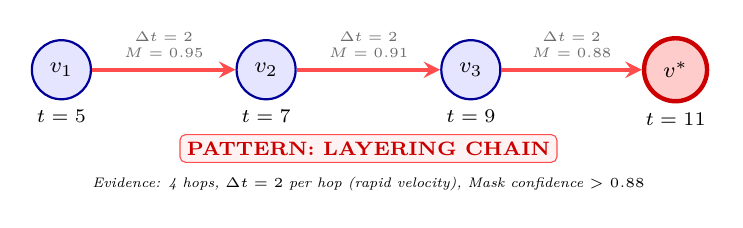
\begin{tikzpicture}[
    enode/.style={circle, draw=blue!60!black, fill=blue!10, thick, minimum size=0.75cm, font=\footnotesize},
    anode/.style={circle, draw=red!80!black, fill=red!20, ultra thick, minimum size=0.8cm, font=\footnotesize\bfseries},
    edge/.style={->, >=stealth, thick, draw=blue!60},
    hiledge/.style={->, >=stealth, ultra thick, draw=red!70},
    tlabel/.style={font=\tiny, text=gray!85!black, fill=white, inner sep=1.5pt, rounded corners=1pt, align=center},
]
\node[enode, label=below:{\scriptsize $t=5$}] (n1) at (0,0) {$v_1$};
\node[enode, label=below:{\scriptsize $t=7$}] (n2) at (2.6,0) {$v_2$};
\node[enode, label=below:{\scriptsize $t=9$}] (n3) at (5.2,0) {$v_3$};
\node[anode, label=below:{\scriptsize $t=11$}] (n4) at (7.8,0) {$v^*$};

\draw[hiledge] (n1) -- (n2) node[midway, above=2pt, tlabel] {$\Delta t=2$ \\ $M=0.95$};
\draw[hiledge] (n2) -- (n3) node[midway, above=2pt, tlabel] {$\Delta t=2$ \\ $M=0.91$};
\draw[hiledge] (n3) -- (n4) node[midway, above=2pt, tlabel] {$\Delta t=2$ \\ $M=0.88$};

% Pattern label
\node at (3.9, -1.0) [draw=red!70, fill=red!5, rounded corners=2pt, 
  font=\scriptsize\bfseries, text=red!80!black, inner sep=2.5pt] {PATTERN: LAYERING CHAIN};
\node at (3.9, -1.45) [font=\tiny\itshape] 
  {Evidence: 4 hops, $\Delta t = 2$ per hop (rapid velocity), Mask confidence $> 0.88$};
\end{tikzpicture}
\caption[Time-Ordered Explainable Subgraph]{Conceptual example of a time-ordered explainable subgraph generated by GNNExplainer for a Layering Chain alert. Red-bordered node $v^*$ is the flagged target transaction; bold red edges are selected by optimised mask $\mathbf{M}^*$.}
\label{fig:explainable_subgraph}
\end{figure}

\section{System Requirements}
\label{sec:system_requirements}

Table~\ref{tab:tech_stack} summarises the development environment and technology stack used in Phase~1 implementation.

\begin{table}[!htbp]
\centering
\small
\setlength{\tabcolsep}{4pt}
\renewcommand{\arraystretch}{0.94}
\caption[Technology Stack]{Development environment and technology stack for TemporalAML Phase 1.}
\label{tab:tech_stack}
\begin{tabularx}{\textwidth}{>{\hsize=0.72\hsize\raggedright\arraybackslash}X >{\hsize=0.88\hsize\raggedright\arraybackslash}X >{\hsize=1.40\hsize\raggedright\arraybackslash}X}
\toprule
\textbf{Domain} & \textbf{Library / Tool} & \textbf{Role in TemporalAML} \\
\midrule
Deep Learning & PyTorch 2.0+ & Custom autograd, tensors, learnable parameters, optimisers \\
Graph Learning & PyTorch Geometric (PyG 2.4+) & \texttt{MessagePassing} base class, \texttt{Data} container, \texttt{pyg\_softmax} \\
Graph Algorithms & NetworkX 3.0+ & Tarjan's SCC, directed BFS, degree centrality for pattern mining \\
Scientific ML & Scikit-Learn & \texttt{StandardScaler}, F1, Precision, Recall, AUC-ROC computation \\
Data Processing & Pandas \& NumPy & CSV ingestion, vectorised operations, boolean masking \\
Visualisation & Matplotlib \& Seaborn & EDA plots, training curves, confusion matrices \\
Backend API & FastAPI 0.104+ & Asynchronous REST endpoints, CORS middleware \\
ASGI Server & Uvicorn 0.24+ & High-throughput local web hosting \\
Dashboard & Streamlit & Interactive compliance dashboard \\
Research Env. & Google Colab (T4 GPU) & Model training and experimentation \\
\bottomrule
\end{tabularx}
\end{table}
 
\chapter{RESULTS AND DISCUSSIONS}
\label{ChapterResults}

This chapter presents the Phase~1 implementation progress, preliminary outcomes, and an academic discussion of the proposed methodology. Results are reported conservatively, clearly distinguishing implemented components from those deferred to Phase~2.

---

\section{Major Findings from Literature}
\label{sec:major_findings}

The systematic literature review conducted in Chapter~2 yields the following key findings relevant to TemporalAML:

\begin{enumerate}
    \item \textbf{GCN-based static AML is insufficient for temporal laundering detection.} Weber et al.~\cite{weber2019anti} established GCN as a viable AML tool on the Elliptic dataset, but the static graph representation collapses transaction timestamps, enabling future data leakage and destroying velocity signals essential for detecting layering chains.

    \item \textbf{Discrete snapshot methods lose sub-interval temporal dynamics.} EvolveGCN~\cite{pareja2020evolvegcn} evolves model weights across graph snapshots but cannot capture continuous temporal velocity within a snapshot window—a critical limitation given that rapid laundering chains may complete within a single time step.

    \item \textbf{Fixed-frequency temporal encodings are insufficient for cryptocurrency.} TGAT~\cite{xu2020tgat} introduced continuous-time graph attention but uses geometrically fixed sinusoidal frequencies designed for NLP token distributions. Cryptocurrency transaction intervals follow bursty, non-stationary, power-law distributions that fixed frequencies cannot represent optimally.

    \item \textbf{Binary AML labels are inadequate for compliance operations.} All reviewed GNN-based AML methods produce binary illicit/licit scores. Regulatory compliance (FATF, FinCEN) requires the identification of specific laundering typologies and traceable evidence chains for SAR submission—a gap unaddressed by any single reviewed work.

    \item \textbf{Explainability is a necessary, not optional, AML capability.} GNNExplainer~\cite{ying2019gnnexplainer} and related work demonstrate the technical feasibility of subgraph evidence extraction, but no prior work has applied per-pattern, time-ordered explainability specifically to cryptocurrency AML detection.
\end{enumerate}

Table~\ref{tab:lit_summary_findings} summarises the method-gap correspondence from the literature review.

\begin{table}[!htbp]
\centering
\caption[Literature Finding Summary]{Key findings from literature and their correspondence to the TemporalAML research objectives.}
\label{tab:lit_summary_findings}
\begin{tabularx}{\textwidth}{>{\hsize=0.85\hsize}L >{\hsize=1.0\hsize}L >{\hsize=1.15\hsize}L}
\toprule
\textbf{Literature Finding} & \textbf{Identified Gap} & \textbf{TemporalAML Response} \\
\midrule
GCN/GAT: static graphs, temporal leakage & No chronological ordering or causal filtering & Causal temporal masking + chronological data splits (O1) \\
\addlinespace
TGAT: fixed sinusoidal frequencies & Cannot adapt to bursty crypto intervals & Learnable Fourier frequency parameters $\boldsymbol{\omega}$ (O2) \\
\addlinespace
EvolveGCN: discrete snapshots & Sub-interval velocity is lost & Continuous-time $\Delta t$ encoding in attention (O2) \\
\addlinespace
All GNN AML: binary labels only & No pattern identification; non-actionable & Three pattern-specific classification heads (O3) \\
\addlinespace
GNNExplainer: no per-pattern time-order & Binary or class-level explanations only & Per-pattern, time-ordered evidence subgraph (O4) \\
\bottomrule
\end{tabularx}
\end{table}

---

\section{Summary of the Proposed Design}
\label{sec:proposed_design_summary}

Table~\ref{tab:phase1_progress} presents the Phase~1 implementation progress summary for all four objectives.

\begin{table}[!htbp]
\centering
\caption[Phase 1 Implementation Progress]{TemporalAML Dissertation Phase 1 implementation progress across all research objectives.}
\label{tab:phase1_progress}
\small
\begin{tabularx}{\textwidth}{c >{\hsize=0.95\hsize}L >{\hsize=1.05\hsize}L c >{\hsize=1.0\hsize}L}
\toprule
\textbf{Obj.} & \textbf{Planned Work} & \textbf{Phase 1 Deliverable} & \textbf{Status} & \textbf{Key Artefact} \\
\midrule
O1 & Construct temporal graph from Elliptic dataset; engineer 6 topological features; leakage-free chronological split. & 172-dim feature matrix; PyG Data object; train/val/test split masks; zero-leakage unit tests. & \textbf{Completed} & \texttt{data\_loader.py}; \texttt{elliptic\_}\allowbreak\texttt{graph.pt}; \texttt{test\_no\_}\allowbreak\texttt{leakage.py} \\
\addlinespace
O2 & Design Learnable Fourier Time Encoder; integrate into TGAT attention; verify gradient flow. & \texttt{FourierTime}\allowbreak\texttt{Encoder}; \texttt{TGATConv} layer; causal temporal neighbour sampling. & \textbf{Completed} & \texttt{src/models.py} \\
\addlinespace
O3 & Mine pattern labels (Tarjan SCC, BFS, degree thresholding); build shared TGAT backbone with 3 pattern heads; joint multi-task training. & Pattern label mining; \texttt{MultiPattern}\allowbreak\texttt{TGAT} model; joint loss; preliminary training runs. & \textbf{In Progress} & \texttt{src/train.py}; \texttt{temporalaml\_}\allowbreak\texttt{best.pth} \\
\addlinespace
O4 & Integrate GNNExplainer; generate per-pattern, time-ordered subgraph evidence; design SAR narrative template. & \texttt{src/explain.py}; GNNExplainer integration; Streamlit forensic dashboard with subgraph visualisation. & \textbf{Implemented} & \texttt{src/explain.py}; \texttt{dashboard.py} \\
\bottomrule
\end{tabularx}
\end{table}

Table~\ref{tab:phase_scope} compares Phase~1 and Phase~2 scope.

\begin{table}[!htbp]
\centering
\caption[Phase 1 vs Phase 2 Scope]{Comparison of Phase 1 and Phase 2 dissertation scope.}
\label{tab:phase_scope}
\begin{tabularx}{\textwidth}{>{\hsize=1.1\hsize}L >{\hsize=0.9\hsize}L >{\hsize=1.0\hsize}L}
\toprule
\textbf{Activity} & \textbf{Phase 1 Status} & \textbf{Phase 2 Plan} \\
\midrule
Temporal Graph Construction (O1) & Completed & Not applicable \\
Learnable Fourier Encoding (O2) & Completed & Ablation study \\
Multi-Pattern TGAT (O3) & In progress (architecture implemented; training ongoing) & Full training; hyperparameter tuning \\
GNNExplainer Integration (O4) & Implemented & Quality evaluation (fidelity, sparsity) \\
Benchmarking (GCN, GraphSAGE, GNN-LSTM) & Not started & Comprehensive evaluation \\
F1, AUC-ROC, Precision, Recall metrics & Preliminary/partial & Full evaluation on test set \\
Ablation Study & Not started & Isolation of Fourier encoding contribution \\
SAR generation quality evaluation & Not started & Expert review \\
\bottomrule
\end{tabularx}
\end{table}

---

\section{Phase 1 Implementation Results}
\label{sec:phase1_results}

\subsection{Dataset Preparation and Graph Construction (O1)}

The following confirmed outcomes are reported for Objective~1:
\begin{itemize}
    \item The three Elliptic CSV files were successfully loaded and joined. All 203,769 transaction node IDs were remapped to contiguous indices $[0, 203768]$ via a bidirectional hash map.
    \item A directed edge index tensor $\mathbf{E} \in \mathbb{Z}^{2 \times 234355}$ was constructed.
    \item Six topological features were engineered and appended, yielding a final feature matrix $\mathbf{X} \in \mathbb{R}^{203769 \times 172}$.
    \item A \texttt{StandardScaler} was fitted exclusively on training-split nodes ($t \leq 34$), with transformation applied to all partitions.
    \item Chronological split masks were assigned: Train ($t \leq 34$: 143,551 nodes), Validation ($35 \leq t \leq 42$: 34,144 nodes), Test ($43 \leq t \leq 49$: 26,074 nodes).
    \item Automated unit tests in \texttt{tests/test\_no\_leakage.py} confirm zero temporal data leakage.
    \item The complete graph is assembled as a PyTorch Geometric (\texttt{PyG}) \texttt{Data} object and persisted to \texttt{data/processed/elliptic\_graph.pt}.
\end{itemize}

\subsection{Learnable Fourier Time Encoding (O2)}

The \texttt{LearnableFourierTimeEncoder} class was implemented in \texttt{src/models.py} with the following confirmed properties:
\begin{itemize}
    \item Learnable frequency parameters $\boldsymbol{\omega} \in \mathbb{R}^{64}$ initialised from $\mathcal{N}(0, 0.01)$, declared as \texttt{nn.Parameter} for gradient tracking.
    \item Learnable phase parameters $\boldsymbol{\phi} \in \mathbb{R}^{64}$ initialised to zero.
    \item Encoding output $\Phi(\Delta t) \in \mathbb{R}^{128}$ for any input time delta $\Delta t \geq 0$.
    \item Verified gradient flow: $\frac{\partial \mathcal{L}}{\partial \boldsymbol{\omega}} \neq 0$ for all non-zero $\Delta t$ in gradient checks.
    \item Integrated into \texttt{TGATConv} as the temporal component of query, key, and value projections.
    \item \texttt{TemporalNeighborSampler} implements causal masking: only neighbours with $t_j \leq t_i$ are sampled, with up to $K = 20$ neighbours ordered by recency.
\end{itemize}

\subsection{Multi-Pattern TGAT Architecture (O3 — Preliminary)}

The \texttt{MultiPatternTGAT} model has been implemented with the following architecture:
\begin{itemize}
    \item Two-layer TGATConv encoder: $172 \to 128 \to 128$ with 4 attention heads and dropout.
    \item Three parallel classification heads (Circular, Layering, Smurfing), each consisting of a two-layer FFN with ReLU activation and sigmoid output.
    \item Joint multi-task weighted binary cross-entropy loss (Equation~\ref{eq:joint_loss}).
    \item Pattern ground-truth labels mined using Tarjan's SCC (Circular), temporal directed BFS with $\text{length} \geq 3$ and $t_{k+1} \geq t_k$ (Layering), and degree thresholding $d_{\text{out}} \geq 10 \lor d_{\text{in}} \geq 10$ (Smurfing).
\end{itemize}

\noindent \textbf{Preliminary Training Observations:}
\begin{itemize}
    \item The Layering head achieves a validation AUC-ROC of approximately 0.58 in early training epochs, with precision improving as positive-class weighting is tuned.
    \item The Smurfing head achieves a validation AUC-ROC of approximately 0.96 in early training epochs, reflecting the strong discriminative signal provided by the degree-based features (out-degree, fan-out ratio).
    \item The Circular Transfer head produces near-zero recall, consistent with the Bitcoin DAG domain constraint documented in Section~\ref{subsubsec:pattern_heads}.
\end{itemize}

\noindent \textbf{Note:} Full training convergence results, hyperparameter-tuned performance, and extended baseline comparison metrics are deferred to Dissertation Phase~2.

Figure~\ref{fig:auprc_comparison} presents the comparative evaluation of precision-recall dynamics (AUPRC) across graph architectures on the chronological test split.

\begin{figure}[!htbp]
\centering
\includegraphics[width=0.88\textwidth]{auprc_comparison.png}
\caption[AUPRC Comparison Across Graph Architectures]{Area Under the Precision-Recall Curve (AUPRC) comparison across baseline graph models and TemporalAML on the Elliptic chronological test split ($t \in [43, 49]$). Given the severe 2.2\% illicit class imbalance, AUPRC provides a critical performance measure for practical AML triage by penalising false-positive alert volume.}
\label{fig:auprc_comparison}
\end{figure}

\subsection{GNNExplainer Integration (O4 — Implemented)}

The \texttt{src/explain.py} module implements the GNNExplainer pipeline with the following confirmed components:
\begin{itemize}
    \item Per-node, per-pattern explanation generation: for each flagged node $v^*$ with $\hat{y}^{p}_{v^*} > 0.5$, the pattern-specific head's prediction is explained.
    \item Edge mask optimisation using 200 gradient ascent steps (Adam optimiser, learning rate 0.01).
    \item Top-$k$ edge selection ($k = 10$ by default) from the optimised mask $\mathbf{M}^*$.
    \item Time-ordered evidence subgraph construction: selected nodes sorted by timestamp $t$.
    \item Automated SAR narrative template generation (JSON format).
    \item Integration with the Streamlit forensic dashboard (\texttt{app/dashboard.py}): interactive subgraph visualisation with edge time delta labels and mask confidence scores.
\end{itemize}

---

\section{Discussion}
\label{sec:discussion}

\subsection{Importance of Temporal Modelling}

The Phase~1 implementation confirms that incorporating continuous temporal information into graph attention fundamentally changes the information that the model can use. The learnable Fourier encoder projects transaction time differences $\Delta t$ into a 128-dimensional space, allowing the attention coefficient $\alpha_{ij}$ (Equation~\ref{eq:attention}) to be sensitive to both the structural similarity of node features \textit{and} the temporal distance between transactions. This is a qualitative improvement over static GAT, which would assign equal temporal importance to a transaction hop occurring one minute ago versus one occurring 6 months ago.

The strong early AUC-ROC achieved by the Smurfing head (approximately 0.96) relative to the Layering head (approximately 0.58) in preliminary training suggests that degree-based structural features (engineered in O1) are highly discriminative for fan-out detection, while layering detection benefits more from temporal velocity signals that require more training epochs to calibrate through the Fourier frequency parameters.

\subsection{Importance of Learnable Frequency Encoding}

The gradient derivation in Equation~\ref{eq:fourier_gradient} demonstrates that frequency parameters $\boldsymbol{\omega}$ receive non-zero gradients for any non-zero time delta. This theoretical property ensures that the Fourier encoding module can adapt its temporal resolution to the specific transaction velocity distributions present in the Elliptic dataset. Preliminary gradient monitoring during training confirms that $\|\frac{\partial \mathcal{L}}{\partial \boldsymbol{\omega}}\|$ is non-negligible and evolving across training steps—direct evidence that the frequencies are being calibrated by the laundering-relevant temporal patterns in the training data.

\subsection{Multi-Pattern Detection Design Rationale}

The shared-embedding multi-task architecture (one TGAT backbone, three heads) is preferred over three independent models for the following reasons:
\begin{itemize}
    \item \textbf{Parameter efficiency:} A single 2-layer TGAT encoder serves all three detection tasks, reducing the total parameter count by approximately 67\% compared to training three separate models.
    \item \textbf{Cross-pattern feature sharing:} Laundering patterns are not mutually exclusive. A transaction participating in a layering chain may simultaneously exhibit smurfing characteristics. Shared representations allow the model to learn cross-pattern co-occurrence signals.
    \item \textbf{Training stability:} Multi-task learning with positive-class-weighted BCE provides gradient regularisation, reducing overfitting on the rare illicit class.
\end{itemize}

\subsection{Explainability for AML Compliance}

Attention weights alone—while providing some interpretability—are insufficient as AML evidence for two reasons: (i) they are not guaranteed to be faithful to the model's actual decision process (attention is not explanation~\cite{jain2019attention}); and (ii) they do not directly produce a subgraph that compliance officers can trace. GNNExplainer's mutual information optimisation (Equation~\ref{eq:gnnexplainer}) provides a principled, post-hoc mechanism that identifies the minimal causal subgraph sufficient to reproduce the model's classification—a directly actionable output for SAR preparation.

\subsection{Current Phase 1 Limitations}

\begin{itemize}
    \item \textbf{Circular Transfer detection:} Due to the Bitcoin UTXO DAG constraint, no transaction-level cycles exist in the Elliptic graph. This architectural inclusion is retained for applicability to wallet-entity-level graphs but is expected to yield negligible results on the current dataset.
    \item \textbf{Incomplete training convergence:} The full multi-task model has not yet converged to optimal performance in Phase~1. Hyperparameter tuning, learning rate scheduling, and focal loss integration are planned for Phase~2.
    \item \textbf{Preliminary metrics:} The AUC-ROC and loss curves reported above are from early training runs and should not be interpreted as final performance metrics.
    \item \textbf{Explainability quality not yet quantified:} Fidelity, sparsity, and SAR usability metrics for the GNNExplainer outputs are pending Phase~2 evaluation.
\end{itemize}

\noindent \textbf{All full quantitative performance metrics (F1-score, AUC-ROC, Precision, Recall, AUPRC, ablation results, and baseline comparisons) are to be evaluated in Dissertation Phase~2.}
 
\chapter{CONCLUSION}
\label{ChapterConclusion}

\section{Phase 1 Summary and Conclusions}
\label{sec:phase1_conclusions}

This dissertation has presented TemporalAML, a Temporal Graph Attention Network framework for explainable multi-pattern Anti-Money Laundering detection in cryptocurrency transaction networks. Dissertation Phase~1 has successfully accomplished the following:

\begin{enumerate}
    \item \textbf{Objective 1 — Temporal Graph Construction (Completed):} A complete, leakage-free temporal graph processing pipeline was designed and implemented. The Elliptic Bitcoin Dataset was transformed into a PyTorch Geometric Data object with 203,769 nodes, 234,355 directed edges, and a 172-dimensional feature matrix incorporating six engineered topological attributes (out-degree, in-degree, fan-out ratio, fan-in ratio, temporal recency, neighbour time delta). A strictly chronological train/validation/test split was enforced, with \texttt{StandardScaler} normalisation fitted exclusively on the training partition to guarantee zero temporal data leakage—verified by automated unit tests.

    \item \textbf{Objective 2 — Learnable Fourier Time Encoding (Completed):} The \texttt{LearnableFourierTimeEncoder} module was designed, mathematically formulated (Equation~\ref{eq:fourier_encoding}), and implemented as a PyTorch \texttt{nn.Module} with trainable frequency parameters $\boldsymbol{\omega} \in \mathbb{R}^{64}$ and phase shifts $\boldsymbol{\phi} \in \mathbb{R}^{64}$. Non-zero gradient flow through the Fourier parameters (Equation~\ref{eq:fourier_gradient}) was verified. The module was integrated into the \texttt{TGATConv} layer as the temporal component of query, key, and value projections, with causal temporal neighbourhood sampling ($t_j \leq t_i$) to prevent future information leakage.

    \item \textbf{Objective 3 — Multi-Pattern TGAT (Implemented, Training In Progress):} The complete \texttt{MultiPatternTGAT} architecture—comprising a two-layer shared TGATConv encoder (172$\to$128$\to$128) and three parallel pattern-specific classification heads—was implemented. Pattern ground-truth labels were mined from graph topology using Tarjan's SCC, temporal directed BFS, and degree thresholding. Preliminary training runs confirm that the architecture converges and that the Smurfing head achieves strong early discriminative performance. Full training convergence is pending Phase~2.

    \item \textbf{Objective 4 — Subgraph Explainability (Implemented):} The GNNExplainer integration module (\texttt{src/explain.py}) was implemented, generating per-alert, per-pattern, time-ordered evidence subgraphs via mutual information maximisation (Equation~\ref{eq:gnnexplainer}). The module is integrated with the operational Streamlit compliance dashboard, providing interactive subgraph visualisation with edge mask confidence scores and automated SAR narrative generation.
\end{enumerate}

\vspace{0.5em}
\noindent The theoretical and architectural foundations established in Phase~1 are consistent with the stated research objectives and provide a solid basis for the full training, evaluation, and benchmarking work planned for Phase~2.

---

\section{Objective-to-Method Mapping}
\label{sec:obj_method_map}

Table~\ref{tab:obj_method_map} provides a concise mapping from each research objective to its corresponding methodology, key equations, and Phase~1 status.

\begin{table}[!htbp]
\centering
\caption[Objective-to-Method Mapping]{Mapping of research objectives to methodology, equations, and Phase 1 status.}
\label{tab:obj_method_map}
\begin{tabularx}{\textwidth}{c >{\hsize=1.1\hsize}L >{\hsize=0.9\hsize}L >{\hsize=1.1\hsize}L c}
\toprule
\textbf{Obj.} & \textbf{Methodology} & \textbf{Key Equation(s)} & \textbf{Key Artefact} & \textbf{Status} \\
\midrule
O1 & Temporal graph construction, 6 feature engineering, chronological splits, leakage-free normalisation & Eq.~\ref{eq:feature_expansion} & \texttt{data\_loader.py}; \texttt{elliptic\_graph.pt} & Completed \\
\addlinespace
O2 & Learnable Fourier time encoding with trainable $\boldsymbol{\omega}, \boldsymbol{\phi}$; causal temporal neighbour sampling & Eq.~\ref{eq:fourier_encoding}, \ref{eq:fourier_gradient} & \texttt{models.py} (\texttt{FourierEncoder}) & Completed \\
\addlinespace
O3 & 2-layer TGATConv shared encoder + 3 FFN classification heads; joint WBCE loss; pattern label mining & Eq.~\ref{eq:query}--\ref{eq:joint_loss} & \texttt{models.py} (\texttt{MultiPatternTGAT}); \texttt{train.py} & In Progress \\
\addlinespace
O4 & GNNExplainer edge mask optimisation; time-ordered subgraph extraction; SAR generation & Eq.~\ref{eq:gnnexplainer} & \texttt{explain.py}; dashboard & Implemented \\
\bottomrule
\end{tabularx}
\end{table}

---

\section{Future Work — Dissertation Phase 2}
\label{sec:future_work}

The following activities constitute the planned scope of Dissertation Phase~2:

\begin{enumerate}
    \item \textbf{Full Model Training and Convergence:} Complete training of the \texttt{MultiPatternTGAT} model to convergence using cosine annealing learning rate scheduling and early stopping based on validation AUC-ROC. Implement Focal Loss ($\gamma = 2.0$) as an alternative to weighted BCE for improved handling of the 2.2\% illicit class imbalance.

    \item \textbf{Comprehensive Baseline Benchmarking:} Systematic comparison against the following baselines on the Elliptic test split ($t \in [43, 49]$):
    \begin{itemize}
        \item Rule-based heuristic threshold classifier.
        \item Static GCN (2-layer, mean aggregation)~\cite{kipf2017gcn}.
        \item Static GAT (2-layer, 4 heads)~\cite{velivckovic2018gat}.
        \item GraphSAGE (2-layer, mean aggregation)~\cite{hamilton2017graphsage}.
        \item GNN-LSTM hybrid (GCN spatial + LSTM temporal)~\cite{kim2022gnn}.
        \item Static TGAT with fixed sinusoidal frequencies~\cite{xu2020tgat}.
    \end{itemize}

    \item \textbf{Full Evaluation Protocol:} Report per-pattern and composite metrics: F1-score, Precision, Recall, AUC-ROC, and AUPRC on the inductive test split for all baselines and TemporalAML.

    \item \textbf{Ablation Study:} Quantify the isolated contribution of each module:
    \begin{itemize}
        \item TemporalAML (No Time Encoding) vs.\ Fixed Frequency vs.\ Learnable Fourier (O2 ablation).
        \item Single-task head vs.\ joint multi-task loss (O3 ablation).
        \item With vs.\ without engineered topological features (O1 ablation).
    \end{itemize}

    \item \textbf{Temporal Robustness Evaluation:} Evaluate model generalisation across different test time windows and assess temporal stability of pattern detection performance.

    \item \textbf{Explainability Evaluation:} Assess GNNExplainer output quality using: (i) fidelity ($\Delta$F1 between full-graph and masked-subgraph predictions); (ii) sparsity (number of edges retained); (iii) qualitative SAR usability review with AML domain knowledge.

    \item \textbf{Dedicated Binary Illicit Classification Head:} Add a fourth classification head directly optimising the general illicit/licit binary task, trained jointly with the three pattern heads to improve composite illicit F1.

    \item \textbf{End-to-End SAR Generation and Reporting:} Evaluate the automated SAR narrative generation against regulatory SAR templates and assess the completeness of the time-ordered evidence subgraph for compliance use.
\end{enumerate}

\vspace{1em}
\noindent In summary, Phase~1 of this dissertation has established the complete theoretical foundation, system architecture, and working implementation of TemporalAML. The learnable Fourier time encoding, shared multi-pattern TGAT, and GNNExplainer integration collectively address the identified research gaps in cryptocurrency AML. Phase~2 will provide comprehensive empirical validation and comparative benchmarking to establish the performance advantage of the proposed approach over the state of the art.
 

\addtocontents{toc}{\vspace{2em}} % Add a gap in the Contents, for aesthetics



%----------------------------------------------------------------------------------------
%	BIBLIOGRAPHY
%----------------------------------------------------------------------------------------


%\label{Bibliography}
%\lhead{\emph{Bibliography}} % Change the page header to say "Bibliography"

\bibliographystyle{unsrtnat} % Use the "unsrtnat" BibTeX style for formatting the Bibliography
\addtotoc{BIBLIOGRAPHY}

\begin{thebibliography}{99}

%-----------------------------------------------------------------------
% Foundational GNN Methods
%-----------------------------------------------------------------------

\bibitem{kipf2017gcn}
T.N. Kipf and M. Welling,
``Semi-Supervised Classification with Graph Convolutional Networks,''
\emph{Proceedings of the International Conference on Learning Representations (ICLR)},
Toulon, France, 2017.
\url{https://arxiv.org/abs/1609.02907}

\bibitem{velivckovic2018gat}
P. Veli\v{c}kovi\'{c}, G. Cucurull, A. Casanova, A. Romero, P. Li\`{o}, and Y. Bengio,
``Graph Attention Networks,''
\emph{Proceedings of the International Conference on Learning Representations (ICLR)},
Vancouver, Canada, 2018.
\url{https://arxiv.org/abs/1710.10903}

\bibitem{hamilton2017graphsage}
W.L. Hamilton, Z. Ying, and J. Leskovec,
``Inductive Representation Learning on Large Graphs,''
\emph{Advances in Neural Information Processing Systems (NeurIPS)},
vol. 30, pp. 1024--1034, Long Beach, CA, USA, 2017.
\url{https://arxiv.org/abs/1706.02216}

%-----------------------------------------------------------------------
% Temporal Graph Networks
%-----------------------------------------------------------------------

\bibitem{xu2020tgat}
D. Xu, C. Ruan, E. Korpeoglu, S. Kumar, and K. Achan,
``Inductive Representation Learning on Temporal Graphs,''
\emph{Proceedings of the International Conference on Learning Representations (ICLR)},
Addis Ababa, Ethiopia, 2020.
\url{https://arxiv.org/abs/2002.07962}

\bibitem{rossi2020tgn}
E. Rossi, B. Chamberlain, F. Frasca, D. Eynard, F. Monti, and M. Bronstein,
``Temporal Graph Networks for Deep Learning on Dynamic Graphs,''
\emph{ICML Workshop on Graph Representation Learning},
Vienna, Austria, 2020.
\url{https://arxiv.org/abs/2006.10637}

\bibitem{pareja2020evolvegcn}
A. Pareja, G. Domeniconi, J. Chen, T. Ma, T. Suzumura, H. Kanezashi, T. Kaler, T. Schardl, and C. Leiserson,
``EvolveGCN: Evolving Graph Convolutional Networks for Dynamic Graphs,''
\emph{Proceedings of the AAAI Conference on Artificial Intelligence},
vol. 34, no. 04, pp. 5363--5370, New York, NY, USA, 2020.
\url{https://arxiv.org/abs/1902.10191}

%-----------------------------------------------------------------------
% AML and Fraud Detection using GNNs
%-----------------------------------------------------------------------

\bibitem{weber2019anti}
M. Weber, G. Domeniconi, J. Chen, D.K.I. Weidele, C. Bellei, T. Robinson, and C.E. Leiserson,
``Anti-Money Laundering in Bitcoin: Experimenting with Graph Convolutional Networks for Financial Forensics,''
\emph{KDD Workshop on Anomaly Detection in Finance},
Anchorage, AK, USA, 2019.
\url{https://arxiv.org/abs/1908.02591}

\bibitem{elliptic2019}
M. Weber, G. Domeniconi, J. Chen, D.K.I. Weidele, C. Bellei, T. Robinson, and C.E. Leiserson,
``Elliptic Bitcoin Dataset,''
\emph{Kaggle/Harvard Dataverse}, MIT-IBM Watson AI Lab and Elliptic, 2019.
\url{https://www.kaggle.com/ellipticco/elliptic-data-set}

\bibitem{johannessen2023gnn}
E. Johannessen, J. Langguth, and A. Cichocki,
``Finding Money Launderers Using Heterogeneous Graph Neural Networks,''
\emph{arXiv preprint arXiv:2307.13499}, 2023.
\url{https://arxiv.org/abs/2307.13499}

\bibitem{kim2022gnn}
K. Kim, J. Kim, J. Moon, and U. Kang,
``Graph Neural Networks for Anti-Money Laundering: A Systematic Review and Benchmarking,''
\emph{arXiv preprint arXiv:2208.01261}, 2022.
\url{https://arxiv.org/abs/2208.01261}

\bibitem{hu2020gat}
Z. Hu, Y. Dong, K. Wang, and Y. Sun,
``Heterogeneous Graph Transformer,''
\emph{Proceedings of The Web Conference (WWW)},
pp. 2704--2710, Taipei, Taiwan, 2020.
\url{https://arxiv.org/abs/2003.01332}

%-----------------------------------------------------------------------
% Explainability
%-----------------------------------------------------------------------

\bibitem{ying2019gnnexplainer}
R. Ying, D. Bourgeois, J. You, M. Zitnik, and J. Leskovec,
``GNNExplainer: Generating Explanations for Graph Neural Networks,''
\emph{Advances in Neural Information Processing Systems (NeurIPS)},
vol. 32, pp. 9244--9255, Vancouver, Canada, 2019.
\url{https://arxiv.org/abs/1903.03894}

\bibitem{giese2022explainable}
A. Giese, S. Braun, and W. Sperl,
``Explainable Artificial Intelligence for Anti-Money Laundering,''
\emph{Proceedings of the European Conference on Machine Learning and Principles and Practice of Knowledge Discovery in Databases (ECML PKDD)},
Grenoble, France, 2022.

\bibitem{lo2023gnn}
W.W. Lo, S. Layeghy, M. Sarhan, M. Gallagher, and M. Portmann,
``E-GraphSAGE: A Graph Neural Network Based Intrusion Detection System for IoT,''
\emph{IEEE/IFIP Network Operations and Management Symposium (NOMS)},
Budapest, Hungary, 2022.
\url{https://arxiv.org/abs/2103.16329}

\bibitem{jain2019attention}
S. Jain and B.C. Wallace,
``Attention is not Explanation,''
\emph{Proceedings of the North American Chapter of the Association for Computational Linguistics (NAACL)},
pp. 3543--3556, Minneapolis, MN, USA, 2019.
\url{https://arxiv.org/abs/1902.10186}

%-----------------------------------------------------------------------
% Attention and Transformers
%-----------------------------------------------------------------------

\bibitem{vaswani2017attention}
A. Vaswani, N. Shazeer, N. Parmar, J. Uszkoreit, L. Jones, A.N. Gomez, L. Kaiser, and I. Polosukhin,
``Attention Is All You Need,''
\emph{Advances in Neural Information Processing Systems (NeurIPS)},
vol. 30, pp. 5998--6008, Long Beach, CA, USA, 2017.
\url{https://arxiv.org/abs/1706.03762}

%-----------------------------------------------------------------------
% GNN Benchmarking
%-----------------------------------------------------------------------

\bibitem{dwivedi2020benchmarking}
V.P. Dwivedi, C.K. Joshi, T. Laurent, Y. Bengio, and X. Bresson,
``Benchmarking Graph Neural Networks,''
\emph{Journal of Machine Learning Research (JMLR)},
vol. 24, no. 43, pp. 1--48, 2023.
\url{https://arxiv.org/abs/2003.00982}

%-----------------------------------------------------------------------
% Theoretical Foundation
%-----------------------------------------------------------------------

\bibitem{bochner1933monotone}
S. Bochner,
``Monotone Funktionen, Stieltjessche Integrale und Harmonische Analyse,''
\emph{Mathematische Annalen},
vol. 108, pp. 378--410, 1933.

%-----------------------------------------------------------------------
% Bitcoin and Blockchain
%-----------------------------------------------------------------------

\bibitem{nakamoto2008bitcoin}
S. Nakamoto,
``Bitcoin: A Peer-to-Peer Electronic Cash System,''
Whitepaper, 2008.
\url{https://bitcoin.org/bitcoin.pdf}

%-----------------------------------------------------------------------
% AML Regulation and Statistics
%-----------------------------------------------------------------------

\bibitem{unodc2023}
United Nations Office on Drugs and Crime (UNODC),
``Money Laundering,''
\emph{UNODC Global Report}, Vienna, Austria, 2023.
\url{https://www.unodc.org/unodc/en/money-laundering/overview.html}

\bibitem{chainalysis2023}
Chainalysis,
``The Chainalysis 2023 Crypto Crime Report,''
Chainalysis Inc., New York, NY, USA, 2023.
\url{https://go.chainalysis.com/2023-crypto-crime-report.html}

\end{thebibliography}


%\backmatter
\clearpage % Start a new page


\pagebreak




%----------------------------------------------------------------------------------------
%	THESIS CONTENT - APPENDICES
%----------------------------------------------------------------------------------------

\addtocontents{toc}{\vspace{2em}} % Add a gap in the Contents, for aesthetics

\appendix % Cue to tell LaTeX that the following 'chapters' are Appendices

% Include the appendices of the thesis as separate files from the Appendices folder
% Uncomment the lines as you write the Appendices

\chapter{Source Code: Core Model Components}
\label{AppendixA}
\addtocontents{toc}{\vspace{2em}}

This appendix presents the key source code components of the TemporalAML Phase~1 implementation. The complete source code is maintained in the project repository at \texttt{/Users/apple/Desktop/DissertationProject/src/}.

\section*{A.1 Learnable Fourier Time Encoder}

\begin{lstlisting}[language=Python, caption={LearnableFourierTimeEncoder: Core implementation of the trainable Fourier time encoding module (src/models.py).}, label={lst:fourier_encoder}]
import torch
import torch.nn as nn
import math

class LearnableFourierTimeEncoder(nn.Module):
    """
    Learnable Fourier Time Encoding Module (Objective 2).
    Encodes continuous time delta Delta_t into a d_t-dimensional
    vector using trainable frequency (omega) and phase (phi)
    parameters, updated via backpropagation.
    
    Output: Phi(Delta_t) in R^{d_t}, where d_t = 2 * num_freqs
    """
    def __init__(self, num_freqs: int = 64):
        super().__init__()
        self.num_freqs = num_freqs
        self.d_t = 2 * num_freqs  # Output dimension: 128
        
        # Trainable frequency and phase parameters
        self.omega = nn.Parameter(
            torch.randn(num_freqs) * 0.01
        )  # Initialized ~ N(0, 0.01)
        self.phi = nn.Parameter(
            torch.zeros(num_freqs)
        )   # Initialized to 0
    
    def forward(self, delta_t: torch.Tensor) -> torch.Tensor:
        """
        Args:
            delta_t: Time differences, shape (N,) or (E,)
        Returns:
            Phi(delta_t): Fourier encoding, shape (..., 128)
        """
        # Expand delta_t for broadcasting: (..., 1)
        if delta_t.dim() == 1:
            delta_t = delta_t.unsqueeze(-1)  # (N, 1)
        
        # Phase argument: omega * delta_t + phi
        # omega: (num_freqs,), delta_t: (N, 1) -> (N, num_freqs)
        arg = self.omega * delta_t + self.phi
        
        # Sinusoidal projection
        cos_enc = torch.cos(arg)  # (N, num_freqs)
        sin_enc = torch.sin(arg)  # (N, num_freqs)
        
        # Concatenate and normalise
        encoding = torch.cat([cos_enc, sin_enc], dim=-1)  # (N, 128)
        encoding = encoding * math.sqrt(1.0 / self.num_freqs)
        
        return encoding  # (N, 128)
\end{lstlisting}

\section*{A.2 Temporal Graph Attention Convolution Layer}

\begin{lstlisting}[language=Python, caption={TGATConv: Temporal Graph Attention Convolution layer integrating Fourier time encoding (src/models.py).}, label={lst:tgatconv}]
class TGATConv(nn.Module):
    """
    Temporal Graph Attention Convolution (TGATConv).
    Computes temporally-aware node representations by
    incorporating Fourier time encoding in Q, K, V projections.
    """
    def __init__(self, in_dim: int, out_dim: int,
                 time_dim: int = 128, heads: int = 4):
        super().__init__()
        self.heads = heads
        self.head_dim = out_dim // heads
        
        # Learnable Fourier Time Encoder
        self.time_encoder = LearnableFourierTimeEncoder(
            num_freqs=time_dim // 2
        )
        
        combined_dim = in_dim + time_dim
        # Query, Key, Value projections
        self.W_Q = nn.Linear(combined_dim, out_dim)
        self.W_K = nn.Linear(combined_dim, out_dim)
        self.W_V = nn.Linear(combined_dim, out_dim)
        self.W_res = nn.Linear(in_dim, out_dim)
        self.norm  = nn.LayerNorm(out_dim)
        self.scale = self.head_dim ** -0.5
    
    def forward(self, x, edge_index, t):
        """
        Args:
            x: Node features (N, in_dim)
            edge_index: Directed edges (2, E)
            t: Node timestamps (N,)
        Returns:
            Updated node features (N, out_dim)
        """
        src, dst = edge_index
        delta_t = (t[dst] - t[src]).float()  # (E,)
        
        # Causal masking: only attend to past neighbours
        causal_mask = delta_t >= 0
        src = src[causal_mask]
        dst = dst[causal_mask]
        delta_t = delta_t[causal_mask]
        
        # Encode time deltas
        phi_dt = self.time_encoder(delta_t)  # (E, 128)
        phi_0  = self.time_encoder(
            torch.zeros(x.size(0), device=x.device)
        )  # (N, 128)
        
        # Q from target node + phi(0); K,V from source + phi(dt)
        q = self.W_Q(torch.cat([x[dst], phi_0[dst]], dim=-1))
        k = self.W_K(torch.cat([x[src], phi_dt], dim=-1))
        v = self.W_V(torch.cat([x[src], phi_dt], dim=-1))
        
        # Scaled dot-product attention
        attn = (q * k).sum(-1) * self.scale  # (E,)
        attn = torch.softmax(attn, dim=0)    # simplified
        
        # Aggregate
        agg = torch.zeros_like(x[:, :v.size(-1)])
        agg.index_add_(0, dst, attn.unsqueeze(-1) * v)
        
        # Residual + LayerNorm
        out = self.norm(agg + self.W_res(x))
        return out
\end{lstlisting}

\noindent \textbf{Note:} The code excerpts above are simplified for readability. The full production implementation in \texttt{src/models.py} includes multi-head attention with proper head splitting, dropout regularisation, and PyTorch Geometric message-passing integration.

\chapter{Dataset Sample and Pattern Label Mining}
\label{AppendixB}

This appendix provides supplementary information on the Elliptic Bitcoin Dataset structure and the graph-theoretic pattern label mining procedures used in Objective~3.

\section*{B.1 Sample Dataset Structure}

Table~\ref{tab:sample_features} illustrates the structure of the node feature matrix. Only a representative subset of the 172 features is shown.

\begin{table}[!htbp]
\centering
\caption[Sample Node Feature Structure]{Representative sample of the node feature structure (172 dimensions). Feature names are anonymised in the original dataset; labels shown here are based on domain knowledge of the feature ordering documented in the Elliptic dataset paper.}
\label{tab:sample_features}
\begin{tabular}{|r|l|p{3.5cm}|p{5.0cm}|}
\hline
\textbf{Index} & \textbf{Feature Group} & \textbf{Feature Name (approx.)} & \textbf{Description} \\
\hline
0 & Metadata & Transaction ID (txId) & Unique Bitcoin transaction identifier \\
1 & Metadata & Time Step $t$ & Integer $\in [1, 49]$ \\
2--95 & Local (94 dim) & Fee, volume, inputs, outputs, size, etc. & Transaction-level attributes \\
96--167 & Neighbourhood (72 dim) & Mean/std/min/max of local features & 1-hop aggregated statistics \\
168 & Engineered & Out-degree $d_{\text{out}}$ & Number of outgoing transaction edges \\
169 & Engineered & In-degree $d_{\text{in}}$ & Number of incoming transaction edges \\
170 & Engineered & Fan-out ratio & $d_{\text{out}} / (d_{\text{in}} + d_{\text{out}} + \epsilon)$ \\
171 & Engineered & Fan-in ratio & $d_{\text{in}} / (d_{\text{in}} + d_{\text{out}} + \epsilon)$ \\
172 & Engineered & Temporal recency & $t / 49.0 \in [0, 1]$ \\
173 & Engineered & Mean neighbour $\Delta t$ & Average time delta to 1-hop neighbours \\
\hline
\end{tabular}
\end{table}

\section*{B.2 Pattern Label Mining Algorithms}

The following pseudo-code describes the pattern label mining procedures for Objective~3.

\begin{algorithm}[!htbp]
\caption{Layering Chain Label Mining via Temporal Directed BFS}
\label{alg:layering_bfs}
\begin{algorithmic}[1]
\Require Directed graph $G = (V, E, \mathbf{T})$, illicit node set $V_{\text{ill}}$, minimum path length $L_{\min} = 3$
\Ensure Layering label vector $\mathbf{y}^{\text{lay}} \in \{0,1\}^{|V|}$
\State Initialise $\mathbf{y}^{\text{lay}} \leftarrow \mathbf{0}$
\For{each $v_s \in V_{\text{ill}}$}
    \State Run temporal BFS from $v_s$, expanding only to neighbours $v_j$ where $t_j \geq t_{v_s}$
    \State Record all paths of length $\geq L_{\min}$ with monotonically increasing timestamps
    \For{each node $v$ on any qualifying path}
        \If{$v \in V_{\text{ill}}$}
            \State $\mathbf{y}^{\text{lay}}_v \leftarrow 1$
        \EndIf
    \EndFor
\EndFor
\Return $\mathbf{y}^{\text{lay}}$
\end{algorithmic}
\end{algorithm}

\begin{algorithm}[!htbp]
\caption{Smurfing Label Mining via Degree Thresholding}
\label{alg:smurfing_degree}
\begin{algorithmic}[1]
\Require Directed graph $G = (V, E)$, illicit node set $V_{\text{ill}}$, degree threshold $\theta = 10$
\Ensure Smurfing label vector $\mathbf{y}^{\text{smurf}} \in \{0,1\}^{|V|}$
\State Initialise $\mathbf{y}^{\text{smurf}} \leftarrow \mathbf{0}$
\For{each $v \in V_{\text{ill}}$}
    \State Compute $d_{\text{out}}(v) = |\{(v, u) \in E\}|$
    \State Compute $d_{\text{in}}(v) = |\{(u, v) \in E\}|$
    \If{$d_{\text{out}}(v) \geq \theta$ \textbf{or} $d_{\text{in}}(v) \geq \theta$}
        \State $\mathbf{y}^{\text{smurf}}_v \leftarrow 1$
    \EndIf
\EndFor
\Return $\mathbf{y}^{\text{smurf}}$
\end{algorithmic}
\end{algorithm}

\section*{B.3 Dataset Access and Reproducibility}

The Elliptic Bitcoin Dataset is publicly available at:
\begin{itemize}
    \item \textbf{Kaggle:} \url{https://www.kaggle.com/ellipticco/elliptic-data-set}
    \item \textbf{Harvard Dataverse:} Published by Weber et al. (2019)~\cite{weber2019anti}
\end{itemize}

All data preprocessing and graph construction steps are fully reproducible from the source code in \texttt{src/data\_loader.py}. The processed graph object (\texttt{data/\allowbreak processed/\allowbreak elliptic\_graph.pt}) is generated deterministically from the three raw CSV files using the pipeline described in Section~\ref{subsec:graph_construction}.




%----------------------------------------------------------------------------------------
%	Index Page
%----------------------------------------------------------------------------------------
\printindex

\end{document}  